% -*- Mode:TeX -*-

%% IMPORTANT: The official thesis specifications are available at:
%%            http://libraries.mit.edu/archives/thesis-specs/
%%
%%            Please verify your thesis' formatting and copyright
%%            assignment before submission.  If you notice any
%%            discrepancies between these templates and the 
%%            MIT Libraries' specs, please let us know
%%            by e-mailing thesis@mit.edu

%% The documentclass options along with the pagestyle can be used to generate
%% a technical report, a draft copy, or a regular thesis.  You may need to
%% re-specify the pagestyle after you \include  cover.tex.  For more
%% information, see the first few lines of mitthesis.cls. 

%\documentclass[12pt,vi,twoside]{mitthesis}
%%
%%  If you want your thesis copyright to you instead of MIT, use the
%%  ``vi'' option, as above.
%%
%\documentclass[12pt,twoside,leftblank]{mitthesis}
%%
%% If you want blank pages before new chapters to be labelled ``This
%% Page Intentionally Left Blank'', use the ``leftblank'' option, as
%% above. 

%% I took twoside out of the document class statement, and it eliminated the extra blank pages. I hope this is okay.
\documentclass[12pt, twoside]{mitthesis}
\usepackage{lgrind}
\usepackage{graphicx}
\usepackage{url}
\usepackage{hyperref}
\usepackage{doi}
\usepackage{subfig}
\usepackage{floatrow}
% Table float box with bottom caption, box width adjusted to content
\newfloatcommand{capbtabbox}{table}[][\FBwidth]
%\usepackage{epstopdf}
%% These have been added at the request of the MIT Libraries, because
%% some PDF conversions mess up the ligatures.  -LB, 1/22/2014
\usepackage{cmap}
\usepackage[T1]{fontenc}
\pagestyle{plain}

%% This bit allows you to either specify only the files which you wish to
%% process, or `all' to process all files which you \include.
%% Krishna Sethuraman (1990).

% Enter file names to process, (chap1,chap2 ...), or `all' to 
% process all files:
%\typein[\files]{all}
%\def\all{all}
%\ifx\files\all \typeout{Including all files.} \else \typeout{Including only \files.} \includeonly{\files} \fi

\begin{document}

% -*-latex-*-
% 
% For questions, comments, concerns or complaints:
% thesis@mit.edu
% 
%
% $Log: cover.tex,v $
% Revision 1.8  2008/05/13 15:02:15  jdreed
% Degree month is June, not May.  Added note about prevdegrees.
% Arthur Smith's title updated
%
% Revision 1.7  2001/02/08 18:53:16  boojum
% changed some \newpages to \cleardoublepages
%
% Revision 1.6  1999/10/21 14:49:31  boojum
% changed comment referring to documentstyle
%
% Revision 1.5  1999/10/21 14:39:04  boojum
% *** empty log message ***
%
% Revision 1.4  1997/04/18  17:54:10  othomas
% added page numbers on abstract and cover, and made 1 abstract
% page the default rather than 2.  (anne hunter tells me this
% is the new institute standard.)
%
% Revision 1.4  1997/04/18  17:54:10  othomas
% added page numbers on abstract and cover, and made 1 abstract
% page the default rather than 2.  (anne hunter tells me this
% is the new institute standard.)
%
% Revision 1.3  93/05/17  17:06:29  starflt
% Added acknowledgements section (suggested by tompalka)
% 
% Revision 1.2  92/04/22  13:13:13  epeisach
% Fixes for 1991 course 6 requirements
% Phrase "and to grant others the right to do so" has been added to 
% permission clause
% Second copy of abstract is not counted as separate pages so numbering works
% out
% 
% Revision 1.1  92/04/22  13:08:20  epeisach

% NOTE:
% These templates make an effort to conform to the MIT Thesis specifications,
% however the specifications can change.  We recommend that you verify the
% layout of your title page with your thesis advisor and/or the MIT 
% Libraries before printing your final copy.
\title{Effect of self-irradiation damage on thermal diffusivity and SAW speed in a thorium-doped lead sulfide thin film}

\author{Keldin Nehmovitch Sergheyev}
% If you wish to list your previous degrees on the cover page, use the 
% previous degrees command:
%       \prevdegrees{A.A., Harvard University (1985)}
% You can use the \\ command to list multiple previous degrees
%       \prevdegrees{B.S., University of California (1978) \\
%                    S.M., Massachusetts Institute of Technology (1981)}
\department{Department of Nuclear Science and Engineering}

% If the thesis is for two degrees simultaneously, list them both
% separated by \and like this:
% \degree{Doctor of Philosophy \and Master of Science}
\degree{Bachelor of Science in Nuclear Science and Engineering}

% As of the 2007-08 academic year, valid degree months are September, 
% February, or June.  The default is June.
\degreemonth{February}
\degreeyear{2019}
\thesisdate{February 8, 2019}

%% By default, the thesis will be copyrighted to MIT.  If you need to copyright
%% the thesis to yourself, just specify the `vi' documentclass option.  If for
%% some reason you want to exactly specify the copyright notice text, you can
%% use the \copyrightnoticetext command.  
%\copyrightnoticetext{\copyright IBM, 1990.  Do not open till Xmas.}

% If there is more than one supervisor, use the \supervisor command
% once for each.
\supervisor{Michael P. Short}{Assistant Professor of Nuclear Science and Engineering}

% This is the department committee chairman, not the thesis committee
% chairman.  You should replace this with your Department's Committee
% Chairman.
\chairman{Michael P. Short}{Assistant Professor of Nuclear Science and Engineering\\Chairman, NSE Committee for Undergraduate Students}

% Make the titlepage based on the above information.  If you need
% something special and can't use the standard form, you can specify
% the exact text of the titlepage yourself.  Put it in a titlepage
% environment and leave blank lines where you want vertical space.
% The spaces will be adjusted to fill the entire page.  The dotted
% lines for the signatures are made with the \signature command.
\maketitle

% The abstractpage environment sets up everything on the page except
% the text itself.  The title and other header material are put at the
% top of the page, and the supervisors are listed at the bottom.  A
% new page is begun both before and after.  Of course, an abstract may
% be more than one page itself.  If you need more control over the
% format of the page, you can use the abstract environment, which puts
% the word "Abstract" at the beginning and single spaces its text.

%% You can either \input (*not* \include) your abstract file, or you can put
%% the text of the abstract directly between the \begin{abstractpage} and
%% \end{abstractpage} commands.

% First copy: start a new page, and save the page number.
\cleardoublepage
% Uncomment the next line if you do NOT want a page number on your
% abstract and acknowledgments pages.
% \pagestyle{empty}
\setcounter{savepage}{\thepage}
\begin{abstractpage}
% $Log: abstract.tex,v $
% Revision 1.1  93/05/14  14:56:25  starflt
% Initial revision
% 
% Revision 1.1  90/05/04  10:41:01  lwvanels
% Initial revision
% 
%
%% The text of your abstract and nothing else (other than comments) goes here.
%% It will be single-spaced and the rest of the text that is supposed to go on
%% the abstract page will be generated by the abstractpage environment.  This
%% file should be \input (not \include 'd) from cover.tex.
Lead sulfide (PbS) is an important semiconductor for infrared light detection, and its use in space necessitates an understanding of how it evolves when damaged by ionizing radiation. Previous work in chemical bath deposition (CBD) resulted in thin films of epitaxially grown polycrystalline PbS uniformly doped with radioactive thorium 228 (Th-228), permitting convenient study of a self-irradiating sample. This thesis represents a continuation of that work by studying the evolution of thermal diffusivity and surface acoustic wave (SAW) speed in a self-irradiating PbS thin film using the non-contact, non-destructive transient grating spectroscopy (TGS) assay. Radiation damage is allowed to accumulate and TGS is used to take measurements before and after annealing. Damage was presumed to create new phonon-scattering defects, thus decreasing SAW speed and thermal diffusivity. However, after annealing, radiation damage caused a monotonic increase in both. Both parameters asymptotically approach a maximum, which indicates a radiation damage saturation point. Thermal diffusivity does not return to its pre-annealed value, indicating an unknown effect. A longer TGS study is recommended to eliminate latent effects, as well as a band gap time-evolution study and an x-ray diffraction study.

\end{abstractpage}

% Additional copy: start a new page, and reset the page number.  This way,
% the second copy of the abstract is not counted as separate pages.
% Uncomment the next 6 lines if you need two copies of the abstract
% page.
% \setcounter{page}{\thesavepage}
% \begin{abstractpage}
% % $Log: abstract.tex,v $
% Revision 1.1  93/05/14  14:56:25  starflt
% Initial revision
% 
% Revision 1.1  90/05/04  10:41:01  lwvanels
% Initial revision
% 
%
%% The text of your abstract and nothing else (other than comments) goes here.
%% It will be single-spaced and the rest of the text that is supposed to go on
%% the abstract page will be generated by the abstractpage environment.  This
%% file should be \input (not \include 'd) from cover.tex.
Lead sulfide (PbS) is an important semiconductor for infrared light detection, and its use in space necessitates an understanding of how it evolves when damaged by ionizing radiation. Previous work in chemical bath deposition (CBD) resulted in thin films of epitaxially grown polycrystalline PbS uniformly doped with radioactive thorium 228 (Th-228), permitting convenient study of a self-irradiating sample. This thesis represents a continuation of that work by studying the evolution of thermal diffusivity and surface acoustic wave (SAW) speed in a self-irradiating PbS thin film using the non-contact, non-destructive transient grating spectroscopy (TGS) assay. Radiation damage is allowed to accumulate and TGS is used to take measurements before and after annealing. Damage was presumed to create new phonon-scattering defects, thus decreasing SAW speed and thermal diffusivity. However, after annealing, radiation damage caused a monotonic increase in both. Both parameters asymptotically approach a maximum, which indicates a radiation damage saturation point. Thermal diffusivity does not return to its pre-annealed value, indicating an unknown effect. A longer TGS study is recommended to eliminate latent effects, as well as a band gap time-evolution study and an x-ray diffraction study.

% \end{abstractpage}

\cleardoublepage

\section*{Acknowledgments}
I would like to express my sincere gratitude:

To Tzvi Templeman, for generously providing the samples that made this research possible;

To Cody Dennett, for hours and hours of assistance with transient grating spectroscopy;

To Professor Mike Short, for his patience, flexibility, counsel, boundless enthusiasm, and persistent belief that I could do more than I thought I could;

To Professor Dennis Whyte, for his long-term support, guidance, refreshing positivity, and sense of humor;

To Diane Wuesthoff, for providing a foundation and home for me;

To George Luo, for his ongoing investment in me and my education, and his model of self-examination;

To Elaine Skowronski, for loving me at my worst and repeatedly reminding me of my best;

To Kenyon Hood, for hacking through the thicket eleven years before me. Like the four minute mile or landing on the Moon, I knew it could be done because I had seen it done;

To Cameron Hood, for sharing ideas that, over three years, I would reject, then tolerate, then adopt, then advocate;

To Natasha Skowronski, for being the most honorable opponent in disagreement, and my best friend during the hardest years of my life,

And to Lily Rush Olson, for being my champion, my efficiency muse, my assertiveness coach, and my loving partner. You saw me across the finish line, and you thanked \emph{me} for it.

%%%%%%%%%%%%%%%%%%%%%%%%%%%%%%%%%%%%%%%%%%%%%%%%%%%%%%%%%%%%%%%%%%%%%%
% -*-latex-*-

% Some departments (e.g. 5) require an additional signature page.  See
% signature.tex for more information and uncomment the following line if
% applicable.
% % -*- Mode:TeX -*-
%
% Some departments (e.g. Chemistry) require an additional cover page
% with signatures of the thesis committee.  Please check with your
% thesis advisor or other appropriate person to determine if such a 
% page is required for your thesis.  
%
% If you choose not to use the "titlepage" environment, a \newpage
% commands, and several \vspace{\fill} commands may be necessary to
% achieve the required spacing.  The \signature command is defined in
% the "mitthesis" class
%
% The following sample appears courtesy of Ben Kaduk <kaduk@mit.edu> and
% was used in his June 2012 doctoral thesis in Chemistry. 

\begin{titlepage}
\begin{large}
This doctoral thesis has been examined by a Committee of the Department
of Chemistry as follows:

\signature{Professor Jianshu Cao}{Chairman, Thesis Committee \\
   Professor of Chemistry}

\signature{Professor Troy Van Voorhis}{Thesis Supervisor \\
   Associate Professor of Chemistry}

\signature{Professor Robert W. Field}{Member, Thesis Committee \\
   Haslam and Dewey Professor of Chemistry}
\end{large}
\end{titlepage}


\pagestyle{plain}
  % -*- Mode:TeX -*-
%% This file simply contains the commands that actually generate the table of
%% contents and lists of figures and tables.  You can omit any or all of
%% these files by simply taking out the appropriate command.  For more
%% information on these files, see appendix C.3.3 of the LaTeX manual. 
\tableofcontents
\newpage
\listoffigures
\newpage
\listoftables


%% This is an example first chapter.  You should put chapter/appendix that you
%% write into a separate file, and add a line \include{yourfilename} to
%% main.tex, where `yourfilename.tex' is the name of the chapter/appendix file.
%% You can process specific files by typing their names in at the 
%% \files=
%% prompt when you run the file main.tex through LaTeX.
\chapter{Introduction}
Since the very beginning, ionizing radiation has been known by its effects on matter. R\"{o}ntgen deduced the existence of x-rays from fluorescence in a chemically treated piece of cardboard, and Curie deduced that uranium ore caused the accumulation of charge on her electrometer. Not long after, scientists initiated the study of radiation damage by measuring changes in the mechanical properties of metals after being exposed. Now, in the age of semiconductors, similar work has been carried out by dozens of scientists to characterize semiconductor changes after irradiation. The present work represents an installment in this effort by studying material property changes in polycrystalline lead sulfide (PbS) as a result of self-irradiation.

The semiconductor lead sulfide, and thin films thereof, have attracted interest for several reasons. Because PbS has a direct band gap of .41 eV at 300 K, it finds use first and foremost as a detector of infrared light \cite{Machol1993, Machol1994}. This stands in contrast to other detection schemes, which are usually sensitive to heat, and only detect IR indirectly through local heating. These methods must therefore also be careful to reject noise caused by non-infrared sources of heat \cite{Rogalski2012}. In one particularly important application, satellites can be equipped with PbS based sensors to look back on earth to detect the hot ejecta from nuclear missile launches \cite{Rogalski2012}, or to peer into outer space in the service of sub-millimeter astronomy \cite{Baddiley1977}. Without the shielding of earth's atmosphere, instruments in orbit are exposed to considerably more ionizing radiation from the sun and outer space.

While this makes for perhaps the most concrete reason to study radiation damage in lead sulfide, the unusual properties of lead sulfide, as well as the other lead chalcogenides PbSe and PbTe, have stimulated plenty of study and hinted at much untapped technological potential. Consider:
\begin{enumerate}
\item Small direct band gaps that decrease with hydrostatic pressure and, 
\item In contrast to all other compound semiconductors, increase with temperature;
\item Dielectric constants that are unusually large when compared to other semiconductors;
\item Relatively large exciton Bohr radii, enabling tunable quantum confinement effects at relatively large grain sizes;
\item Rock salt crystal lattices that are relatively stable over non-stoichiometry. \cite{Kumar2003}.
\end{enumerate}

These properties have been exploited to make infrared lasers \cite{Malyarevich2000}, solar control coatings \cite{Nair1989}, and even a method of nucleotide detection for DNA sequencing \cite{Hu2009}. Through band gap tuning, PbS may find use in visible light detectors or solar cells \cite{Semonin2012}, and pending a clearer understanding of radiation damage, could be used in fission or fusion reactor instrumentation \cite{Biton2014}. 


% Speculative future applications of PbS(Th) include integrated circuit elements with an expiration date, or elements that require time to enter their operational zone. 





%Of course, anything in orbit is exposed to much more radiation from the sun and outer space than on the earth's surface due to less shielding from the earth's atmosphere. Much of this is ionizing radiation, which is capable of causing material damage, including in lead sulfide detectors. The present work is thus a continuation of efforts to study how lead sulfide responds to radiation damage.

%In particular, efforts at Ben-Gurion University of the Negev by Templeman et al. to grow thin films of lead sulfide by chemical bath deposition (CBD) culminated in development of a novel means to study radiation damage in PbS sulfide by doping the semiconductor with thorium. The radioactive thorium, uniformly dispersed throughout the lattice, destroys lead sulfide's crystal structure over time by blasting it with alpha particles. Templeman et al. studied the evolution of the semiconductor's electrical resistivity as a result of accumulated radiation damage. They demonstrated that resistivity increased up to a maximum and could be undone by annealing.

%The same thorium-doped PbS thin film samples prepared and studied by Templeman et al. made their way to the United States. And in the present work, they are used to study the evolution of thermal diffusivity as a result of accumulated radiation damage using transient grating spectroscopy.



% other cool things about PbS


% radiation damage in PbS
% all the reasons listed by Templeman

% why study radiation damage in semiconductors? 
% 		All electronics exposed to radiation (space, nuclear); expiring ICs; ICs that need time to become functional; ICs that exploit soft errors to generate random numbers.

% why study radiation damage? 
% 		Space, nuclear applications




% thin film
% epitaxial growth - get the same orientation & crystal structure
% homoepitaxial - you get a more perfect crystal than what you started with
% You couldn't grow a crystal otherwise
% you can make layers, like in microchips, thus creating really tiny transistors, etc
% The thinness allows for tuning properties
% why thin films here? because that's just the way they could make PbS that was doped with thorium


% it's important that it's PbS and that it's doped with thorium, but the CBD isn't important. It's just the only way the doping could be done.

% band gap tuning
% radiation damage changes the band gap
% self-destructive electronics
% DNA sequencing with bulk PbS
% 
% Does my sample count as epitaxial because it was grown on GaAs?








% \cite{patterson:risc,rad83}.  
% \cite{ellis:bulldog,pet87,coutant:precision-compilers}.  In these cases, the
% \cite{gib86}.
% These optimizations are described in detail in section~\ref{ch1:opts}.
% \section{Description of micro-optimization}\label{ch1:opts}
% \footnote{A description of the floating point format used is shown in figures~\ref{exponent-format}
% and~\ref{mantissa-format}.}.  
% A discussion of the mathematics behind unnormalized arithmetic is in appendix~\ref{unnorm-math}.

% \footnote{Using unnormalized numbers for math is not a new idea; a
% good example of it is the Control Data CDC 6600, designed by Seymour Cray.
% \cite{thornton:cdc6600} The CDC 6600 had all of its instructions performing
% unnormalized arithmetic, with a separate {\tt NORMALIZE} instruction.}.

% This is an example of how you would use tgrind to include an example
% of source code; it is commented out in this template since the code
% example file does not exist.  To use it, you need to remove the '%' on the
% beginning of the line, and insert your own information in the call.
%
%\tagrind[htbp]{code/pmn.s.tex}{Post Multiply Normalization}{opt:pmn}

% This is an example of how you would use tgrind to include an example
% of source code; it is commented out in this template since the code
% example file does not exist.  To use it, you need to remove the '%' on the
% beginning of the line, and insert your own information in the call.
%
%\tgrind[htbp]{code/be.s.tex}{Block Exponent}{opt:be}

\chapter{Background}
%
% lead sulfide important - study everything about it. Also it's in space. Study radiation damage.
% BGU made a thing. They studied it some. Let's study it some more.
% TGS has been happening at MIT. This is just the next thing we can study it with.
% There's a search for model radiation damage systems.
This work is the result of three separate avenues of progress that happened to converge. They are summarized here and elaborated upon later:
\begin{enumerate}
	\item Recent work to hone chemical bath deposition of PbS culminated in growing thin films of PbS doped with thorium.\label{first_avenue}
	\item Transient grating spectroscopy (TGS) is an emerging tool for studying radiation damage, and its suitability for studying thin films, whether semiconductor or otherwise, has become apparent.\label{second_avenue}
	\item Radiation materials scientists are interested in teasing apart the different radiation damage mechanisms and determining the contribution of each to changes in bulk parameters (such as Young's modulus, strength, resistivity, etc.). Thorium doped PbS holds promise as a ``model system'' for studying radiation damage.\label{third_avenue}
\end{enumerate}
This work defies intuition without understanding that it serves three separate needs simultaneously. 

In Templeman et al. 2017, a team at Ben-Gurion University announced successful doping of a lead sulfide thin film with radioactive Th-228, which they hailed as a new ``model system'' for radiation damage studies. Earlier papers from the same team do not hint that radiation damage studies were their ultimate goal. For instance, Templeman et al. 2014 is simply about the effect of pH and the order of reagent addition on the growth of lead selenide \cite{Templeman2014}. At some point, however, the team realized that doping PbS with Th-228 was worthy of pursuit, and several papers clearly build toward this goal. In particular, Biton et al. 2014 explicitly sets out to alloy PbS with the more common and less radioactive Th-232 in preparation for using Th-228 later \cite{Biton2014}.

Semiconductors and their responses to radiation damage are worthy of study, but an obvious and widely available choice like bulk silicon requires a beam line or reactor. For Si, \emph{in situ} or self-irradiation studies do not make for an easier alternative. One cannot simply add radioactive material to a silicon crystal and isolate the effect of the radiation from the effect of a foreign species in the crystal lattice.\footnote{Hence the pains taken by the BGU team to determine whether thorium could indeed be alloyed with PbS without disturbing the lattice. They confirmed thorium was distributed throughout, and the absence of any phases other than rock salt PbS. \cite{Templeman2017}} Furthermore, radioactive materials are in shorter and more controlled supply than semiconductor materials, so the choice of radioactive material actually comes first, and the choice of semiconductor follows.

Thorium 232 is widely available, and thorium 228 happens to be one of its more active daughters, so it is a perfectly reasonable choice of radioisotope. It also makes sense in light of the BGU team's previous experience with growth of lead chalcogenide thin films: lead is the closest stable nucleus to thorium (or any of the naturally occurring radioisotopes), and lead is the final stable daughter of the thorium decay chain. In summary, though Th-228 is not the only possible choice of radioisotope, and PbS is not the archetypical semiconductor, they make sense together.

Once this line of reasoning is accepted, chemical bath deposition (CBD) as a technique and thin films as a product---rather than bulk materials---are simply consequences. Given current techniques of deposition and alloying, growing crystalline or polycrystalline PbS with a controlled quantity of Th-228 uniformly dispersed throughout necessitates CBD. And CBD, while in theory capable of producing thicker-than-thin films, is essentially only used for making thin films, especially in the case of PbS. In summary, dispersing Th-228 in the PbS crystal requires CBD, and CBD produces thin films.

The discussion so far amounts to an understanding of the present work in the context of the first avenue of progress mentioned above (\ref{first_avenue}). For the third (\ref{third_avenue}), the exciting component is the band gap and quantum confinement features of lead sulfide. The promise of semiconductors doped with radioactive materials as ``model systems'' for studying radiation damage stems from the hope that certain types of radiation damage will have different, distinguishable effects on band gap, grain size, and grain boundary \cite{Templeman2017}; all packaged in a sample that produces very little biologically damaging radiation and requires no handling restrictions \cite{Templeman2017}. By analyzing these material parameters over time, it is hoped that the accumulation and evolution of each type of damage can be better understood. For instance, we know that dislocation loops take more time and damage to appear, but what if a change in band gap indicated their quantity exactly at any time?

The second avenue of progress (\ref{second_avenue}), dictates the quantities measured in this work. We have established the justification for lead sulfide, for doping with Th-228, for using CBD, and for producing thin-films. But these two lines of thinking would suggest measuring resistivity, band gap, grain size, or energy barrier at grain boundary. Instead, in this work we opt to measure thermal diffusivity and surface acoustic wave (SAW) speed (a proxy for elasticity). Resistivity has already been characterized in this sample by Templeman et al. 2017 \cite{Templeman2017}, so it makes sense to study a different quantity. And though band gap might be a more intuitive choice, TGS makes it exceedingly easy to study thermal diffusivity and SAW speed. These quantities are not beside the point because they too convey important information about energy levels in the band gap affecting charge carrier mobility and the presence of defects to scatter phonons.

% If just interested in thermal diffusivity, then why report about elasticity? Because TGS
% If just interested in TGS, then why study BGU? Because they made it.
% If just interested in model material, why not measure band gap? Because TGS
% if just interested in radiation damage in PbS, then why not use bulk? Because this is uniformly damaging.


\section{Semiconductor physics and prediction}
In metals, electrical conductivity and thermal conductivity are seemingly linked; an observation that is formalized in the Wiedemann-Franz relation,
\begin{equation}
\frac{\kappa}{\sigma} = LT.
\end{equation}
Although not exactly true, this relationship holds because electrical and thermal conductivity in metals are both dominated by the same parameter: the high mobility of charge carriers, i.e. electrons \cite{Lavasani2018}. The effect of radiation damage on electrical and thermal conductivity can thus be understood in terms of its effect on electron mobility. The story for semiconductors becomes more complicated.

It is still true that electrical conductivity depends on the concentration of charge carriers and the mobility of charge carriers:
\begin{equation}
\sigma = en_p\mu_h + en_e\mu_e.
\end{equation}
But in semiconductors, density of charge carriers is no different than a metal or any other material of similar atomic number, and instead mobility of charge carriers becomes the limiting factor.

Concerning thermal conductivity, there are two mechanisms: charge carriers and phonons. Phonons, the quasi-particles that represent the solid's normal vibrational modes, are a means of thermal conductivity in metals as well, but their contribution is small compared to that of charge carriers. In semiconductors, because the charge carrier mobility is low, the phonon contribution matters.

So, in semiconductors, electrical conductivity is governed by charge carrier mobility, but thermal conductivity is governed by charge carrier mobility and phonon transport. This is why something like the Wiedemann-Franz relation does not exist for semiconductors, and is why we cannot expect radiation damage to have the same effect on thermal conductivity as it does on electrical conductivity.
% semiconductor: thermal diffusivity depends on charge carriers and also phonon transport. Metals have this too, it's just that phonons barely matter. Anyway, phonons scatter off defects.
% semiconductor: electrical conductivity depends on charge carrier mobility
% 
%[Needs rearranging]

The key defining feature of the semiconductor is the band gap: the region of forbidden electron energy and momentum levels between the material's valence and conduction bands. In order to conduct, an electron must absorb a minimum amount of energy and momentum to jump the gap, leaving behind a positively charged ion: a "hole". The electron remains in the conduction band until it finds a hole to recombine with; relaxing back to the valence band by releasing a photon.

We therefore expect radiation damage to affect charge carrier mobility through introducing new energy levels into the band gap, thus reducing the energy necessary for conduction. We expect radiation damage to affect phonon transport through creation of defects, leading to more phonon scattering. For thermal diffusivity, it is not clear which of these hypothesized mechanisms should dominate, since more charge carrier mobility would tend to increase thermal diffusivity and more phonon scattering should reduce thermal diffusivity. Since phonon transport dominates without radiation damage, we expect that reducing this quantity will dominate, and thermal diffusivity will be reduced by damage. For SAW speed, only phonon transport can have an effect, since SAWs can be thought of mathematically as low frequency phonons. Therefore, radiation damage ought to decrease SAW speed. This also satisfies intuition, since crystals in general have higher SAW speeds than amorphous materials.

%[More to say]

%Any semiconductor that starts neutral thus contains an equal number of electrons and holes at all times.

%[Orphan paragraph:]
%The direct band gap of lead sulfide means that, unlike better known semiconductors like silicon, the closest approach between the valence band and the conduction band, energy-wise, does not require any momentum. This makes it conceptually simpler than many semiconductors, but momentum still plays a roll in lead sulfide's thermal properties.
%
%[Orphan paragraph:]
%Usually, electrons in semiconductors acquire the momentum they need to conduct from the solid's vibrational normal modes, called phonons. Since any arbitrary set of motions of a solid's constituent atoms can be decomposed into a sum of normal modes, all kinetic energy within a solid, from acoustic to thermal, can be thought of as a population of phonons. The lower frequencies are associated with acoustics, and the higher ones with thermal properties. 


%\emph{[Insert figure with band structure (E vs. k) for Si and PbS)]}

%Semiconductor optical, electrical, and thermal behavior always comes down to consideration of mobility of charge carriers, phonon population, and band gap. 

\section{Transient Grating Spectroscopy - TGS}
Transient Grating Spectroscopy (TGS) was developed incrementally, but begins with Cachier's work at the Laboratoire d'Ultrasons in Paris in 1970 \cite{Cachier2003}. Lately, TGS crafted according to the specifications of Johnson et al. 2012 \cite{Johnson2012} was set up at MIT under the auspices of the Mesoscale Nuclear Materials Group \cite{Cometto2018}. TGS enables the determination of a sample's material properties by using lasers to excite and measure the propagation of surface acoustic waves (SAWs). It has a host of advantages as a non-destructive, non-contact, rapid assay; but as a surface to mesoscale depth assay, it is especially appropriate for studying thin films and low-penetration radiation damage.

\begin{figure}[thb]
\begin{center}
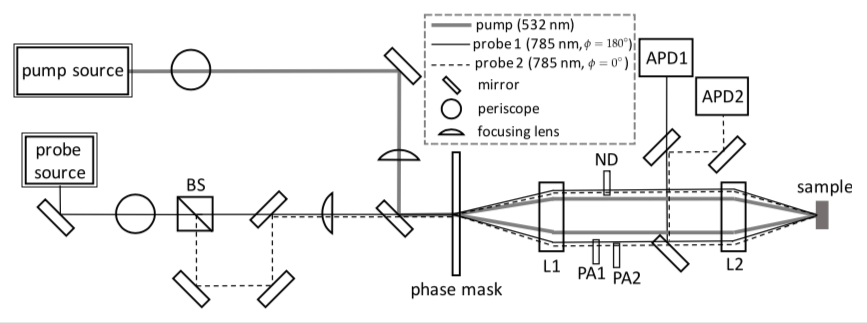
\includegraphics[width=\textwidth]{./images/TGS-DH_setup_Dennet_2017b_1.png}
\caption{Typical TGS setup. L1 and L2 are focusing lenses; ND is a neutral density filter; PA1 and PA2 represent phase adjustments; and APD1 and APD2 are the avalanche photodiodes which collect the reflected probe beam. Image adapted from Dennett and Short 2017 \cite{Dennett2017}.}
\label{TGS_setup}
\end{center}
\end{figure}

Figure \ref{TGS_setup} illustrates a typical TGS setup. Two lasers of the same wavelength $\lambda_{0}$ and phase are aimed at the sample such that the beams overlap and interfere at the sample surface. In this setup, each laser, called a pump beam, mirrors the angle $\theta$ from normal of the other. Both beams are linearly polarized, so where the beams overlap, which we call the footprint, interference will create parallel lines of constructive interference. Where there is constructive interference, the material will experience heating and expansion, uplifting a tiny ripple on the material surface. The lasers are shut off, but the ripples begin to propagate outward and decay as soon as they are created; a process which depends on the material's elasticity and thermal diffusivity. A third laser, called the probe beam, is directed at a fixed location within the footprint, such that the ripples travel beneath it and reflect the probe beam at varying angles. By detecting the reflected beam and its changing angle in avalanche photodiodes, we can deduce the shape and speed of the ripple beneath the probe beam. The resultant signal over time represents the ripples as they travel underneath the probe beam. Refer to Figure \ref{TGS_sample_output}. The oscillations in this curve represent the ripples due the constructive interference of the pump beams; frequency depends on the material's Young's modulus; and time decay depends on the material's thermal diffusivity.

\begin{figure}[thb]
\begin{center}
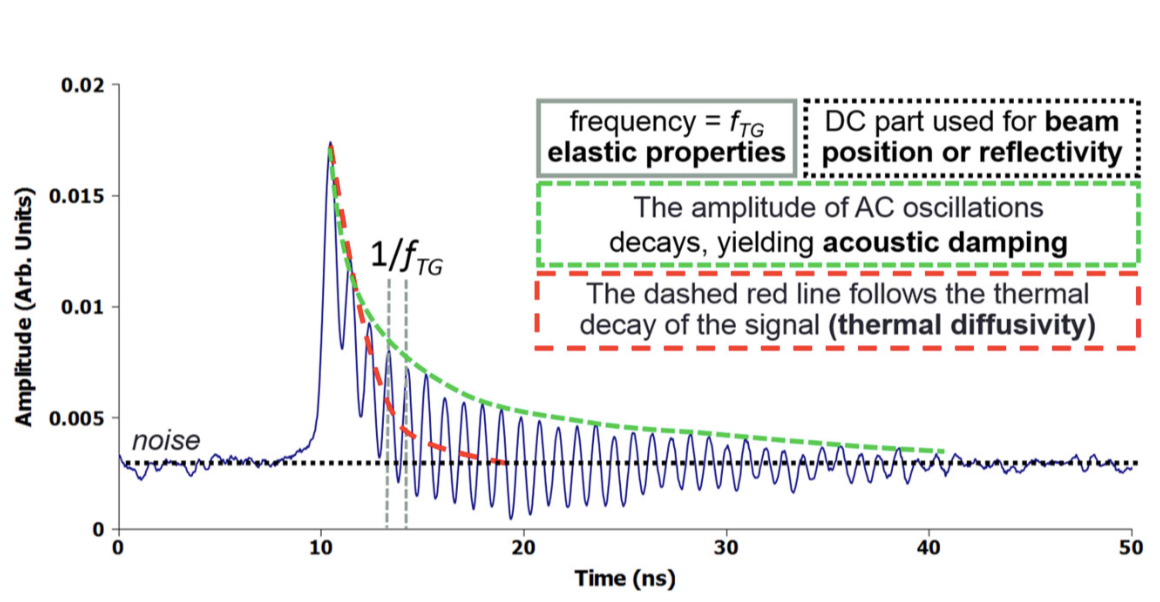
\includegraphics[width=\textwidth]{./images/Sample_TGS_output_2.png}
\caption{Generic TGS output signal plotted with known useful decomposable components called out. Image adapted from Short et al. 2015 \cite{Short2015}.}
\label{TGS_sample_output}
\end{center}
\end{figure}

The ripples continue to the edge of each grain, where they experience some reflection and some transmission to adjacent grains. At the edge of the sample, they reflect. These edge effects can alter the signal picked up by the probe beam, so it is essential that the grain size either be much larger or much smaller than the footprint of the pump lasers. Larger so that reflected waves do not return in time to be recorded; or smaller so that there are enough grains over which to average the grain boundary effect.

If the wavelength of probe beam is $\lambda_0$, then we can expect the wavelength of the ripples of constructive interference to be
$\lambda = \lambda_0 sin(\theta)$, where theta is, again, the angle from normal.

%[Trying to understand how thickness matters. Can a sample be too thin for TGS? Will the GaAs substrate of the PbS(Th) sample have an effect on the results reported from TGS?]

The areas of local heating on the sample surface also penetrate into the material, requiring consideration of the material thickness and desired depth of study. This has an acoustic and thermal component governed by the material speed of sound and the thermal diffusivity, respectively. The acoustic component is therefore roughly immediate and requires that the defects to be studied are within one $\lambda$ of the surface. The thermal component takes longer, and therefore doesn't affect the signal recorded by the probe beam.

In this work, the key consideration is not that the radiation damage is beyond one $\lambda$ from the surface, but rather that the entire thin film is thinner than $\lambda$. The SAW travels parallel to the film-substrate boundary, but the amplitude is such that lead and sulfur atoms will exert pressure on the gallium and arsenic atoms in the substrate. At this boundary, as in all coupled oscillator systems, there is some amount of reflection and transmission of the energy to the substrate. While this affect could be modeled and deconvolved, in this work we assume that since it is present in both the pre-annealing radiation damaged measurements and the post-annealing measurements, it affects all results equally. The thermal diffusivity and SAW speed results should not be expected to match the values of bulk PbS or bulk PbS(Th). Rather, the \emph{percent changes} should match.

\section{Sample preparation}
The thorium doped PbS thin film was prepared by chemical bath deposition (CBD) before the present work began. Templeman et al. 2017 \cite{Templeman2017} describe the process in detail, but it is summarized here for completion. The GaAs (100) substrate was submerged in a chemical bath containing thorium 228. The thorium concentration, temperature, and pH were all precisely varied to control the concentration of thorium incorporated into the PbS rock salt lattice; a method that was confirmed to work by Biton et al. 2014 \cite{Biton2014}. The thorium added to the solution had already aged $\sim$2.5 years since it was created in presumably pure form. Therefore, its daughters were also present in the solution, and Templeman et al. confirmed by gamma and alpha spectroscopy that at least some of the daughters were incorporated into the lattice as well, though they did not attempt to deduce or measure concentrations. The sample properties as reported by Templeman et al. 2017 are collected in Table \ref{sample_properties} and a photo of the sample can be seen in Figure \ref{photo_of_thin_film_sample}.

%\begin{table}[hb]
%\begin{center}
%\begin{tabular}{|l|l|}\hline
%Substrate						&	GaAs (100) \\\hline
%Dimensions					&	1 cm x 1.5 cm \\\hline
%Film thickness					&	$\sim$500 nm \\\hline
%Grain size						&	$\sim$150 nm \\\hline
%Th 228 concentration			&	0.15 ppm \\\hline
%Total activity*					&	65 Bq \\\hline
%Sample creation date			&	22 Jul 2016\\\hline
%\end{tabular}
%\end{center}
%\label{sample_properties}
%\caption{Sample properties reported by Templeman et al. 2017 \cite{Templeman2017}. * Total activity measured a brief but unknown time after sample preparation.}
%\end{table}


\begin{figure}[tbp]
\begin{floatrow}
\ffigbox{%
  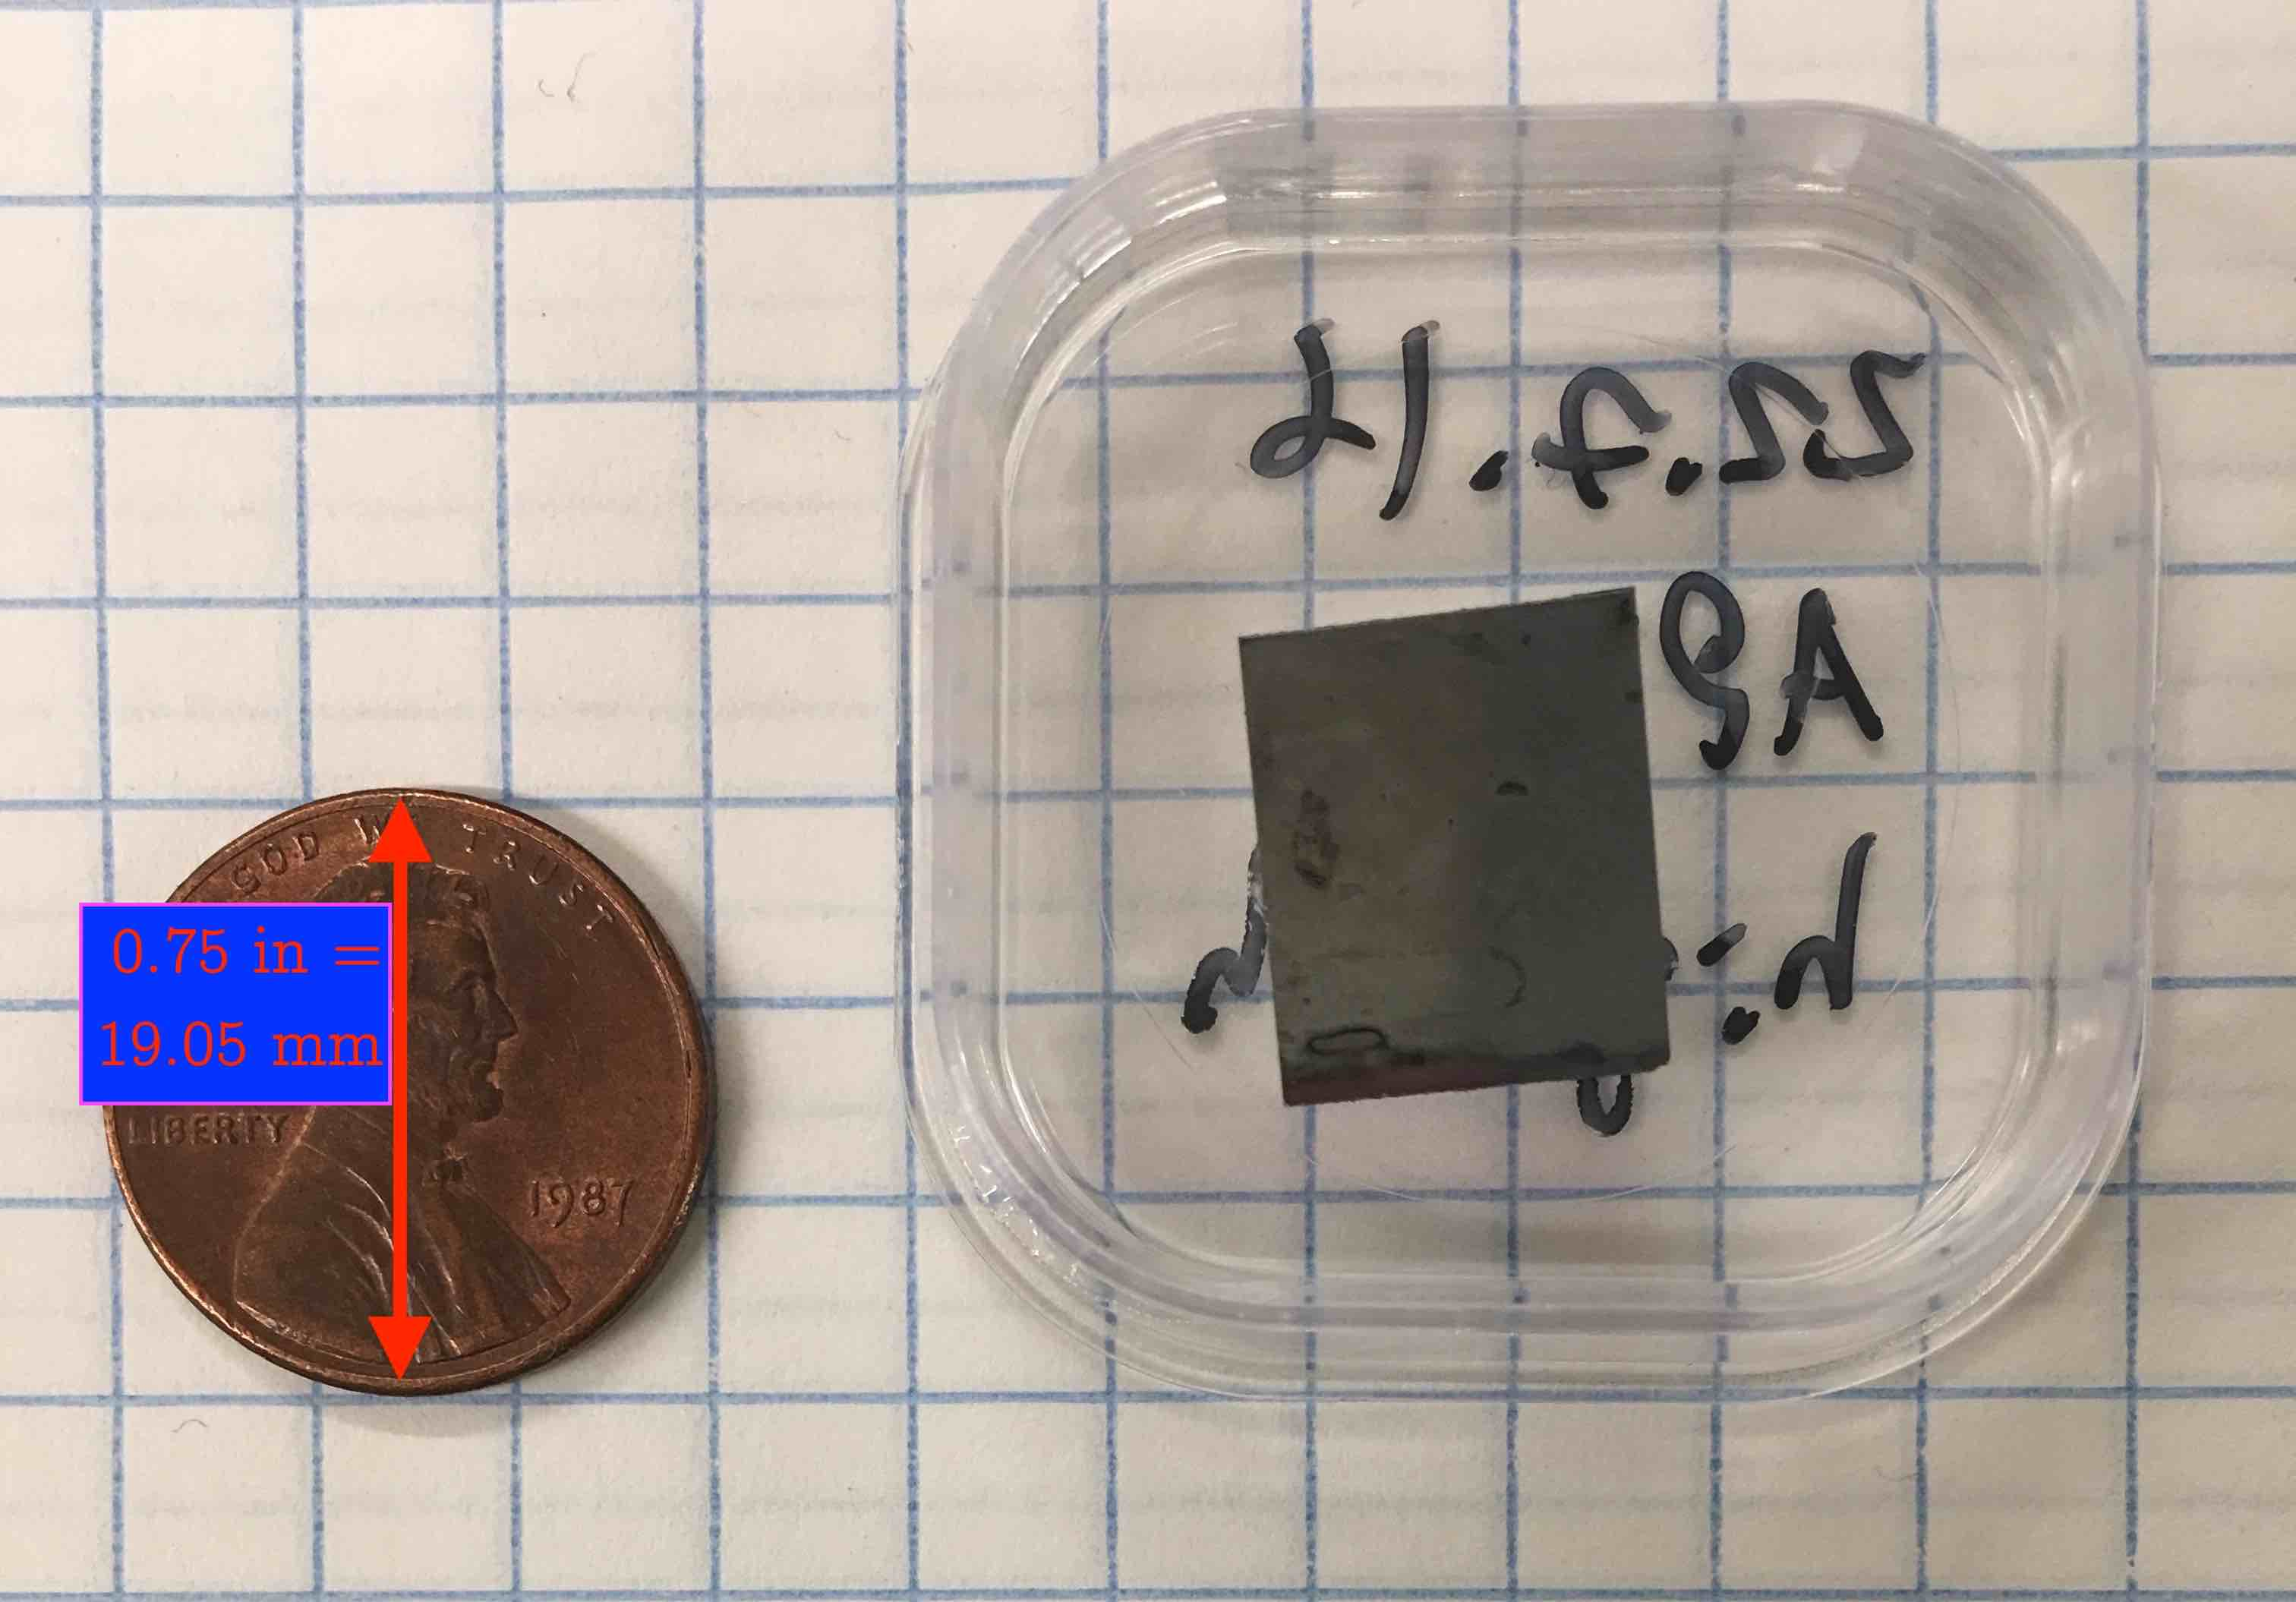
\includegraphics[width=3in]{./images/photo_of_thin_film_sample.jpg}%
}{%
  \caption{Top-down photo of the thin film sample of PbS(Th) analyzed in this work. US penny included for scale.\label{photo_of_thin_film_sample}}%
}
\capbtabbox{%
\begin{tabular}{|l|l|}\hline
Substrate						&	GaAs (100) \\\hline
Dimensions					&	1 cm x 1.5 cm \\\hline
Film thickness					&	$\sim$500 nm \\\hline
Grain size						&	$\sim$150 nm \\\hline
Th 228 concentration			&	0.15 ppm \\\hline
Total activity*					&	65 Bq \\\hline
Sample creation date			&	22 Jul 2016\\\hline
\end{tabular}
}{%
  \caption{Sample properties reported by Templeman et al. 2017 \cite{Templeman2017}. * Total activity measured a brief but unknown time after sample preparation. \label{sample_properties}}%
}
\end{floatrow}
\end{figure}


%[What about crystal misfit calculations? Can I just say that I neglected them, but that PbS and GaAs have pretty different lattice constants and it might actually matter.]

% \cite{patterson:risc,rad83}.  
% \cite{ellis:bulldog,pet87,coutant:precision-compilers}.  In these cases, the
% \cite{gib86}.
% These optimizations are described in detail in section~\ref{ch1:opts}.
% \section{Description of micro-optimization}\label{ch1:opts}
% \footnote{A description of the floating point format used is shown in figures~\ref{exponent-format}
% and~\ref{mantissa-format}.}.  
% A discussion of the mathematics behind unnormalized arithmetic is in appendix~\ref{unnorm-math}.

% \footnote{Using unnormalized numbers for math is not a new idea; a
% good example of it is the Control Data CDC 6600, designed by Seymour Cray.
% \cite{thornton:cdc6600} The CDC 6600 had all of its instructions performing
% unnormalized arithmetic, with a separate {\tt NORMALIZE} instruction.}.

% This is an example of how you would use tgrind to include an example
% of source code; it is commented out in this template since the code
% example file does not exist.  To use it, you need to remove the '%' on the
% beginning of the line, and insert your own information in the call.
%
%\tagrind[htbp]{code/pmn.s.tex}{Post Multiply Normalization}{opt:pmn}

% This is an example of how you would use tgrind to include an example
% of source code; it is commented out in this template since the code
% example file does not exist.  To use it, you need to remove the '%' on the
% beginning of the line, and insert your own information in the call.
%
%\tgrind[htbp]{code/be.s.tex}{Block Exponent}{opt:be}

\chapter{Methods}
%\section{Sample preparation}
%The thorium doped PbS thin film was prepared by chemical bath deposition (CBD) before the present work began. Templeman et al. 2017 \cite{Templeman2017} describe the process in detail, but it is summarized here for completion. The GaAs (100) substrate was submerged in a chemical bath containing thorium 228. The thorium concentration, temperature, and pH were all precisely varied to control the concentration of thorium incorporated into the PbS rock salt lattice; a method that was confirmed to work by Biton et al. 2014 \cite{Biton2014}. The thorium added to the solution had already aged $\sim$2.5 years since it was created in presumably pure form. Therefore, its daughters were also present in the solution, and Templeman et al. confirmed by gamma and alpha spectroscopy that at least some of the daughters were incorporated into the lattice as well, though they did not attempt to deduce or measure concentrations. The sample properties as reported by Templeman et al. 2017 are collected in Table \ref{sample_properties} and a photo of the sample can be seen in Figure \ref{photo_of_thin_film_sample}.
%
%%\begin{table}[hb]
%%\begin{center}
%%\begin{tabular}{|l|l|}\hline
%%Substrate						&	GaAs (100) \\\hline
%%Dimensions					&	1 cm x 1.5 cm \\\hline
%%Film thickness					&	$\sim$500 nm \\\hline
%%Grain size						&	$\sim$150 nm \\\hline
%%Th 228 concentration			&	0.15 ppm \\\hline
%%Total activity*					&	65 Bq \\\hline
%%Sample creation date			&	22 Jul 2016\\\hline
%%\end{tabular}
%%\end{center}
%%\label{sample_properties}
%%\caption{Sample properties reported by Templeman et al. 2017 \cite{Templeman2017}. * Total activity measured a brief but unknown time after sample preparation.}
%%\end{table}
%
%
%\begin{figure}
%\begin{floatrow}
%\ffigbox{%
%  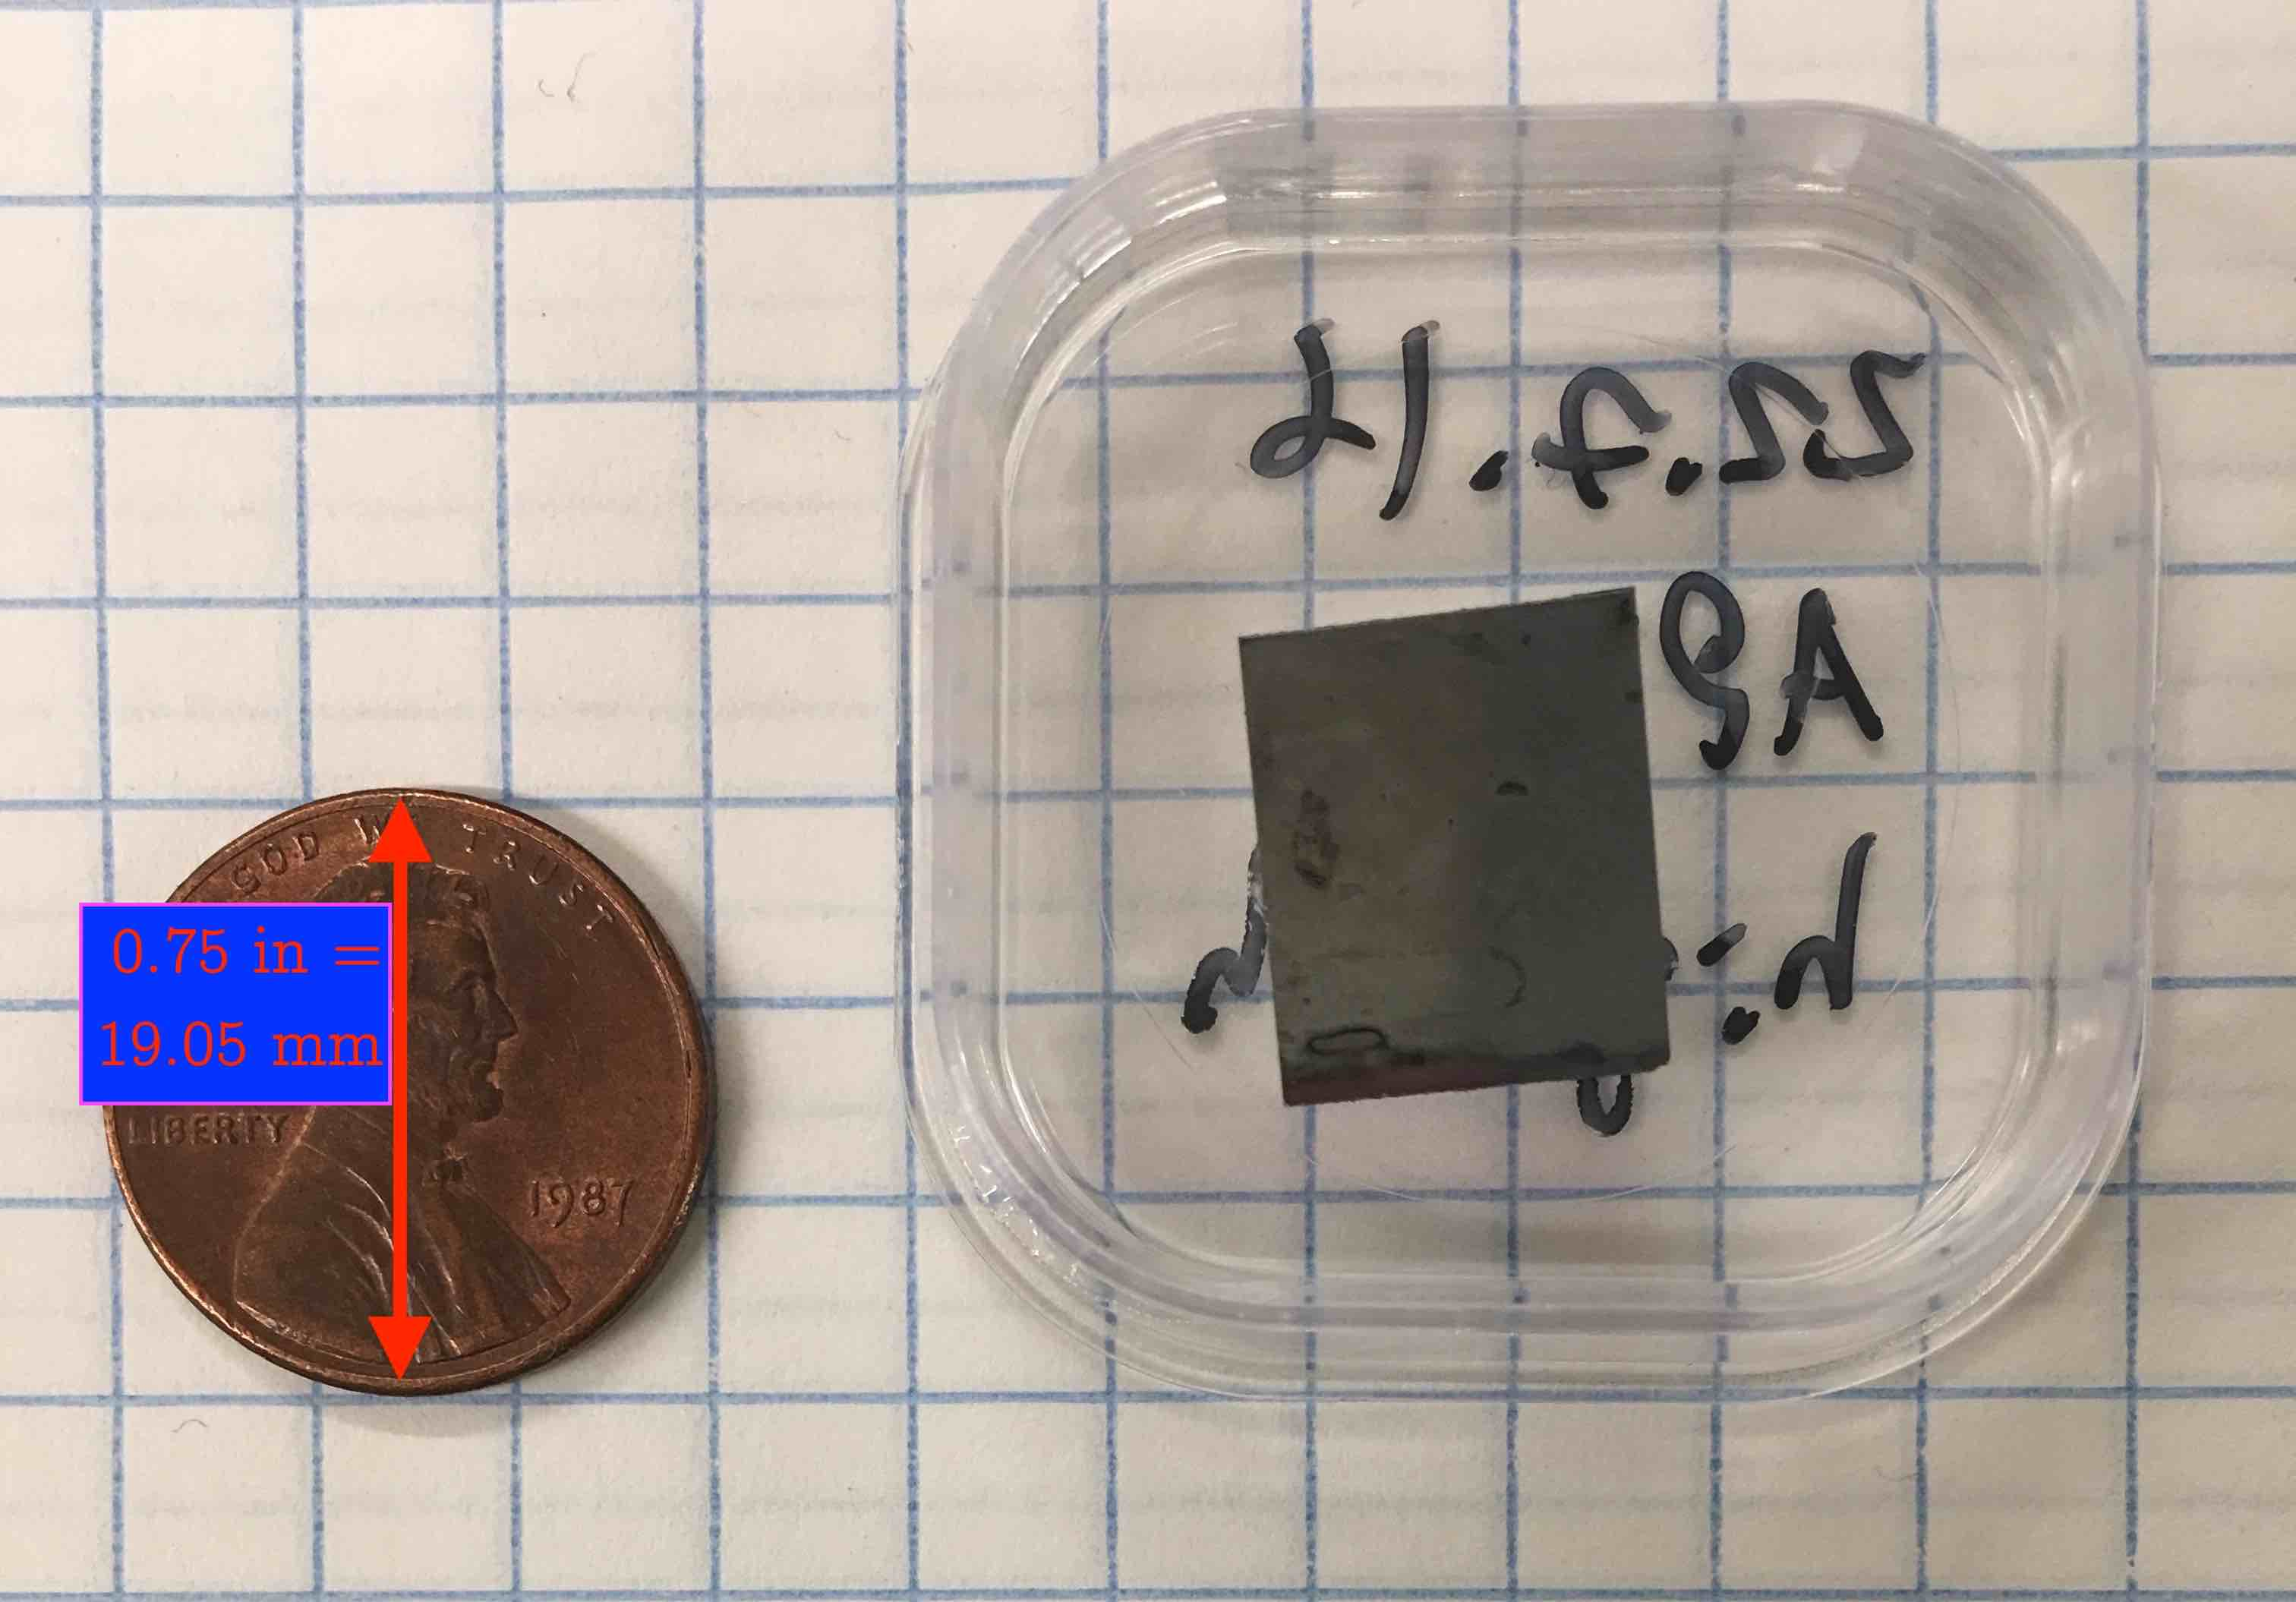
\includegraphics[width=3in]{./images/photo_of_thin_film_sample.jpg}%
%}{%
%  \caption{Top-down photo of the thin film sample of PbS(Th) analyzed in this work. US penny included for scale.\label{photo_of_thin_film_sample}}%
%}
%\capbtabbox{%
%\begin{tabular}{|l|l|}\hline
%Substrate						&	GaAs (100) \\\hline
%Dimensions					&	1 cm x 1.5 cm \\\hline
%Film thickness					&	$\sim$500 nm \\\hline
%Grain size						&	$\sim$150 nm \\\hline
%Th 228 concentration			&	0.15 ppm \\\hline
%Total activity*					&	65 Bq \\\hline
%Sample creation date			&	22 Jul 2016\\\hline
%\end{tabular}
%}{%
%  \caption{Sample properties reported by Templeman et al. 2017 \cite{Templeman2017}. * Total activity measured a brief but unknown time after sample preparation. \label{sample_properties}}%
%}
%\end{floatrow}
%\end{figure}
\section{Transient grating spectroscopy}
838 days elapsed between sample preparation and TGS measurements, which was presumed to be plenty of time for radiation damage to accumulate to a maximum in the sample. After initial calibration runs with tungsten, two sets of runs were conducted with one annealing stage between them. Before annealing, five runs where conducted with the vacuum chamber at <12 mTorr and no temperature control (i.e. roughly room temperature). The annealing was conducted at 280 $^\circ$C and $\sim$15 mTorr for 3 hours. The sample was allowed to cool naturally until it hit 90 $^\circ$C, at which point the chamber was exposed to atmospheric pressure (700 mTorr) to assist cooling. At 30 $^\circ$C, pumping was resumed to evacuate the chamber once again. When the pressure descended below 25 mTorr, 90 post-annealing runs were conducted at 2 minute intervals. The DAQ faulted after 3:02 hrs, so an additional five runs were conducted at 2 minute intervals at about 8mTorr.

\section{TGS Data Analysis}
The mathematical foundation of TGS data analysis is discussed in depth in two papers by Dennett \& Short \cite{Dennett2017, Dennett2018}. These methods were in turn implemented in a library of MATLAB functions in Dennett and Short 2018 and hosted on GitHub \cite{dennett_short_github}. The functions of this library were utilized in ew MATLAB scripts written for this work. All scripts and functions used in this work are publicly available online in a GitHub repository \cite{Sergheyev2019}. Any modifications of the original library from Dennett and Short 2018 can also be found there.

\section{Radiation damage}
\subsection{Decay chain}
The decay chain of thorium 228 was computed with the Universal Decay Calculator, available online \cite{wise_calculator}. Thorium 228 was assumed pure at creation, then aged 913 days ($\approx$2.5 years) before being added, along with its decay products, to the chemical bath solution to grow the PbS thin film. It is assumed that thorium 228 and all of its daughters were incorporated in the to PbS crystal lattice in proportion to the concentrations with which they were present in the chemical bath. For instance, if the ratio of radium 224 to thorium 228 were 2:1 in the chemical bath, then we expect that ratio to hold in the solid solution of the thin film as well. It is not currently known how accurate this assumption is, or if epitaxial growth shows a preference for some daughters on a chemical basis over others.

After the thin film was prepared, its total activity was measured to be 65 Bq, which we can use to extrapolate the activity at the time of the TGS measurements. If we assume this activity of 65 Bq represents the complete inventory of radionuclides in the thin film at $t = 913$ days (i.e. neglecting how different emissions are attenuated differently and detected with different efficiencies), then we can work backward to determine what initial activity of Th-228 must have been on the day it was prepared.

Take as an ansatz that the initial activity of Th-228 was 1.0 Bq when pure at $t=0$. Age it 913 days, and we get a decay chain inventory with total activity 2.843 Bq. Thus, an activity of 22.86 Bq must have been initially present to result in a total activity of 65 Bq at $t=913$. This method was used to compute the inventory at different times, as shown in Table \ref{ansatz_decay_chain_inventory}. The final time, $t=1751$, is the time at which the experiment in this work took place (i.e. TGS and annealing).

\begin{figure}[th]
\begin{center}
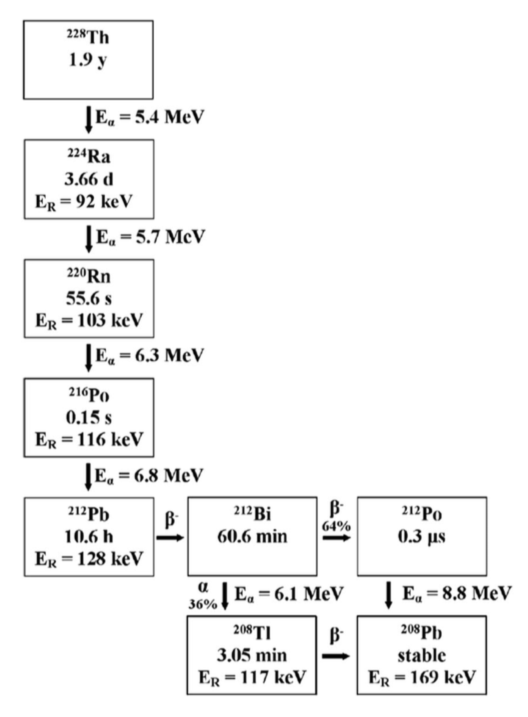
\includegraphics[width=.5\textwidth]{./images/Th_228_decay_chain.png}
\caption{The decay chain of thorium 228 is a subset of the decay chain of the more familiar isotope thorium 232. Shown are the daughters, alpha energies, and daughter recoil energies. Where nuclides are known to emit alphas of more than one energy, the energy shown is an average of all alpha energies weighted by their intensity (i.e. percent of decays)\cite{Templeman2017, CRC}.}
\label{Th_228_decay_chain}
\end{center}
\end{figure}

\begin{figure}[thb]
\begin{center}
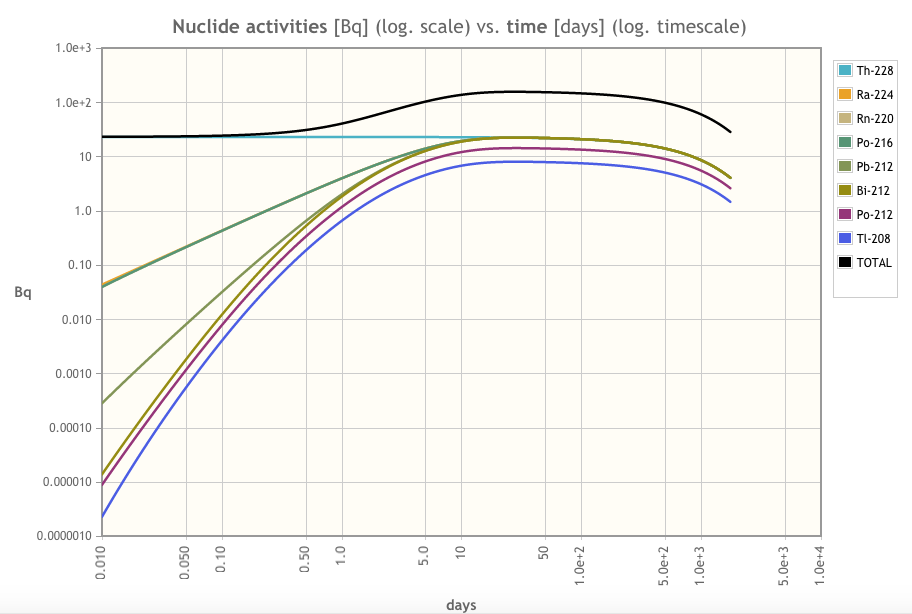
\includegraphics[width=\textwidth]{./images/thorium_decay_chain_plot.png}
\caption{Plot of the time evolution of the Th-228 decay chain inventory, with each species' activity also plotted. $t=0$ is the time of Th-228 preparation. Th-228 activity decreases monotonically, but total activity increases before falling off. Total and all individual activities are declined by the time of sample preparation. All non-stable daughters have shorter half-lives than Th-228, but secular equilibrium with Th-228 is never attained because Pb-212 is more stable than its parent Po-216.}
\label{plot_of_inventory_time_evolution}
\end{center}
\end{figure}


\begin{table}[th]
\begin{center}
\begin{tabular}{|r|c|c|c|}\hline
		&	$t=0$	&	$t=913$	&	$t=1751$	\\\hline
Th-228	&	22.86	&	9.241	&	4.024	\\
Ra-224	&	0		&	9.290	&	4.045	\\
Rn-220	&	0		&	9.290	&	4.045	\\
Po-216	&	0		&	9.290	&	4.045	\\
Pb-212	&	0		&	9.296	&	4.048	\\
Bi-212	&	0		&	9.297	&	4.048	\\
Po-212	&	0		&	5.956	&	2.594	\\
Tl-208	&	0		&	3.340	&	1.454	\\\hline
Total		&	22.86	&	65.00	&	28.30	\\\hline
\end{tabular}
\end{center}
\caption{Computed inventory of complete thorium 228 decay chain at different times: (a) at time of Th-228 preparation; (b) at time of CBD of PbS(Th) thin film; (c) at the time of radiation damage study with TGS. All times given in days and all activities given in Bq \label{ansatz_decay_chain_inventory}}
\end{table}%


\subsection{SRIM/TRIM}
SRIM 2013 \cite{srim_website} was utilized to simulate alpha and recoiling daughter transport in the lead sulfide thin film in order to get an estimate of the damage caused by the decay chain presented above. SRIM, an abbreviation of Stopping and Range of Ions in Matter, is a closed-source suite of programs to perform a number of calculations and simulations related to user specified ions incident upon a user defined material target. In one program, SR, ion range in a target is calculated directly with tabulated values, interpolation, and heuristics. TRIM, which is an abbreviation of Transport of Ions in Matter, uses a monte carlo simulation of probabilistic ion collisions in the material to construct cascades, and thus report on basic damage formation.

SR and TRIM were used first to estimate the range of both alphas and recoiling daughters within PbS(Th), and secondly to estimate the damage rate in DPA/s of the radiation emitted by the thorium decay chain. Input files can be found in the GitHub repository for this work \cite{Sergheyev2019}, but important values used across the SRIM suite are summarized in Table \ref{trim_inputs}.

\begin{table}[thb]
\begin{center}
\begin{tabular}{|r|r|}\hline
Incident alpha energy	&	5423 $keV$\\
Random seed			&	716381\\
Density				&	7.60 $g/cm^3$ \cite{CRC}\\
\# of particles simulated	&	9999\\\hline
\end{tabular}
\begin{tabular}{|r|r|r|r|}\hline
					&	$^{207}$Pb	&	$^{32}$S		&	$^{228}$Th\\\hline
Stoichiometry (ppb)		&	499999925	&	499999925	&	150		\\\hline
Displacement energy (eV)&	16.4			&	16.4			&	16.4 		\\\hline
Lattice binding energy (eV)&	2			&	2			&	2 		\\\hline
Surface binding energy (eV)&	2.2			&	5.63			&	2 		\\\hline
\end{tabular}
\end{center}
\caption{SRIM/TRIM inputs for calculating range of alpha particles in PbS(Th). 5423 keV is the primary alpha from Th-228 decay \cite{NNDC}. The lattice binding energy and surface binding energy are values recommended by SRIM's creators; as is the unusual and unusually specific choice of random seed \cite{srim_textbook}. 16.4 eV represents half of PbS's crystal binding energy \cite{Tanaka1979}.\label{trim_inputs}}
\end{table}%

According to SR, 5.423 MeV alpha particles incident upon an infinite volume of PbS with 15 ppm Th doping ought to have a range of 18.41 $\mu m$ with a straggling of 1.06 $\mu m$. In TRIM, 9999 alphas were simulated in an infinite medium, which resulted in a similar range of 18.4 $\mu m$ with a straggling of 0.7488 $\mu m$. Lateral range was under 2 $\mu m$ in both cases, and therefore negligible. In other words, the alpha particles exhibit typical behavior of traveling in a straight line and coming to an abrupt stop. The significance of the range of the alphas compared to the thickness will be discussed later.

Next, TRIM was used to estimate the damage from alphas. In the infinite volume case, TRIM reports 366 displacements/alpha, 23 of which result in recombination of an interstitial and a vacancy. When the layer thickness was reduced to 500 nm to match the thin film, the displacements/alpha dropped to 2.


% Repo for code: http://dx.doi.org/10.5281/zenodo.1239854 
%
%
% Atmospheric pressure is 760 Torr
% run_notes.txt:
%BGU Experiment
%Sample: "22.7.16 high Th"
%Date: 2018/11/07
%
%- Pre anneal measurements at <12mTorr
%- During the anneal
%- 11:32 30mTorr (right as it hit 280C)
%- 11:35 14mTorr
%- 11:45 10mTorr
%- 12:00 9mTorr
%- 14:31 8mTorr, heater turned off
%- 15:00 crack to air on cool down at 90C
%- 15:09 start to pump again at 30C
%- 15:15 start 4 hour post-anneal @ 25mTorr
%- 15:30 10mTorr
%- bottomed out at 8mTorr again for room temp ost anneal
%
%- Set was four hour post anneal and cool at 5000 traces per batch on 2 minute intervals
%- DAQ faulted after 3 hours and 2 minutes on post_anneal_00
%- Do a series of 5x5000 starting at 19:10ish
%- stop measurement after those 5. 
%- final temperature record saved in "temp_rec_04.csv" for the entire experiment.
%
%
%


\chapter{Results \& Discussion}
Results for radiation damage calculations and simulations are reported and discussed first, followed by results from TGS.

\section{Radiation damage}
In the absence of a dedicated monte carlo code to model the PbS(Th) thin film more accurately, quantifying the radiation damage requires some decisions about which sources of damage can be neglected. The 18.4 $\mu m$ range of alphas in PbS(Th) indicates that alphas traveling in the z-direction (the dimension in which the film is thin) traverse the 500 nm with little resistance and simply exit the sample. On the way, they disturb electrons and create phonons, but cause negligibly few displacements. This is true regardless of where in the sample they are born.

If, however, they are born with a trajectory in the xy plane (the dimensions in which the thin film is 1 cm x 1.5 cm), then the film is plenty large enough for them to deposit all of their energy and cause hundreds of displacements. However, the total solid angle for this situation is small compared with the solid angle of traversing the film in its thinner directions. In other words, most alphas will be born with a location and trajectory that leaves them very little PbS(Th) crystal to traverse before exiting the thin film.

The alpha energy used, 5423 keV, is of course, not the only alpha energy in the Th-228 decay chain. But it does represent the lowest energy/highest interaction alpha of the preferred alpha decays (the alpha which, for a particular nuclide, is emitted most often). As such, this analysis is even more true of the other, more energetic alphas in the decay chain.

This analysis has three important implications. 
\begin{itemize}
\item Damage from radiation with any lower probability of interaction can be neglected. This means gammas and betas, each with smaller interaction cross sections and less energy to deposit, can be neglected.
\item It justifies the assumption made earlier that all radiation produced by thorium decay chain is detectable. The alphas detected in the previous work by Templeman et al. faithfully represent the alphas born in the material, and the activity detected can be assumed to be the activity of the thorium decay chain.
\item The bulk of the radiation damage in the thin film must be a result of recoiling daughters.
\end{itemize}


\section{Thermal diffusivity and SAW speed}
Results are plotted in Figures \ref{thermal_diffusivity_pre_post}, \ref{curve_fit}, \ref{T_P_alpha_subplots}, and \ref{SAW_speeds}.  Figure \ref{thermal_diffusivity_pre_post} shows the thermal diffusivity over time for the duration of the experiment; thus indicating the baseline thermal diffusivity before annealing, and then the post-annealing baseline, followed by a monotonic increase over $\sim$4 hours. 

During the months preceding this experiment, radiation damage was presumed to reach a steady maximum. At this maximum, either the lattice would have become completely amorphous, or an equilibrium would exist whereby additional atomic displacements would be just as likely to create new Frenkel pairs as they would be to cause recombination.

Annealing was expected to heal the accumulated damage, allowing the whole process to begin again. One might expect that damage would \emph{reduce} thermal diffusivity, but that annealing would reset $\alpha$ to a \emph{higher} value associated with phonon transport in a low defect crystal. After annealing, the radiation damage would slowly set in, and TGS results would show the thermal diffusivity declining until it arrived back at the pre-annealing value. Or, if contrary to phonon scattering considerations, radiation damage actually \emph{increased} thermal diffusivity, then annealing would reset it to a \emph{lower} value and TGS would measure radiation damage increasing it. Regardless of what annealing might do to thermal diffusivity, we would expect radiation damage to push thermal diffusivity back to its pre-annealed value.

In brief, these intuitions amount to five primary expectations:
\begin{enumerate}
\item Radiation damage effects over the months preceding this work should have reached a steady state. Each parameter ought to be at an extremum.
\item Annealing should restore each parameter to its pre-irradiation value.
\item Radiation damage should tend to push the parameter back to its steady state value---the value measured prior to annealing.
\item Radiation damage should decrease thermal diffusivity
\item Radiation damage should decrease SAW speed.
\end{enumerate}

Neither thermal diffusivity nor SAW speed behaved entirely as expected.

Refer again to Figure \ref{SAW_speeds}. The data indicates that SAW speed is increased by radiation damage rather than decreased, but the rest of its behavior roughly matches expectation. Annealing pulls SAW speed down, and new radiation damage pushes SAW speed back toward its pre-annealing value.

There is in fact precedent in the literature for this behavior, even if it was not apparent that it was applicable before. In Dienes's 1952 paper and in Nabarro's response, the effect of interstitials and vacancies on elasticity is investigated \cite{Dienes1952a, Nabarro1952}. They conclude that vacancies exert a tensile stress on the material, while interstitials exert a compressive stress. These contributions are not equal and opposite, because interstitials exert an order of magnitude more stress \cite{Dienes1952a}. Their work on metals such as copper and sodium would at first seem not to be applicable because metallic bonds dictate very different response to radiation damage than the covalent bonds present in lead sulfide, but it amounts to a very compelling hypothesis for the results obtained in this work. Perhaps, then, the apparent increase in the maximum SAW speed (as a result of damage) after annealing is due to residual interstitials that did not recombine during annealing. Instead, the atoms around them relaxed, as Dienes describes, which effectively ``bakes'' in the damage. On the second round of radiation, damage and thus stiffness have a head start.

Refer again to Figure  \ref{thermal_diffusivity_pre_post}. The data indicates that annealing increases thermal diffusivity, but so does radiation damage. Since we expected the effect of annealing and the effect of radiation damage to cancel one another, this is very surprising. It is also not clear how the thermal diffusivity got so low as its pre-annealing value if months of radiation damage should have increased it.

Of the two competing mechanisms discussed in the background---increased charge carrier mobility and increased phonon scattering---the data appears to suggest that increased charge carrier mobility is actually dominant effect of radiation damage. Or, at least it does in the short term. There could be both short term and long term effects that are opposing. This could explain the increase in thermal diffusivity over this experiment, while also accounting for a gradual decline months later when the latent effect takes over.

As a final note, in both samples we observe a ``hook'' before the overall post-annealing trend emerges. Since the timing of the hook behavior lines up with the times the chamber was cracked to atmosphere and then re-pumped (see \ref{T_P_alpha_subplots}), it is believe that this behavior is a result of the pressure differential, and not radiation damage. We already know that lead sulfide's band gap is sensitive to pressure, so it makes sense that its other properties would be too. For the purposes of this study, we can treat as comparable only the TGS measurements taken below 15 mTorr.


%Mike Short recommends these:
%G. J. Dienes, A theoretical estimate of the effect of radiation on the elastic constants of simple metals, Phys. Rev. 86, 228 (1952).
%F. R. N. Nabarro, Effect of radiation on elastic constants, Phys. Rev. 87, 665 (1952).
%G. J. Dienes, Effect of radiation on elastic constants, Phys. Rev. 87, 666 (1952).


% hook
% New energy levels in the gap
% Umklapp scattering
% Phonon scattering off defects
% heat? pressure?
% 1) messed up analysis
% 2) messed up experiment
% 3) Annealing problem
% 		delamination, atoms boiling off, phase transition, oxidation, change in grain size
% 4) pressure problem
% 5) 

% why not short term mobility + long term phonon scattering?
% curve is exponential
% resistance should have diminished.



\begin{figure}[pt]
\begin{center}
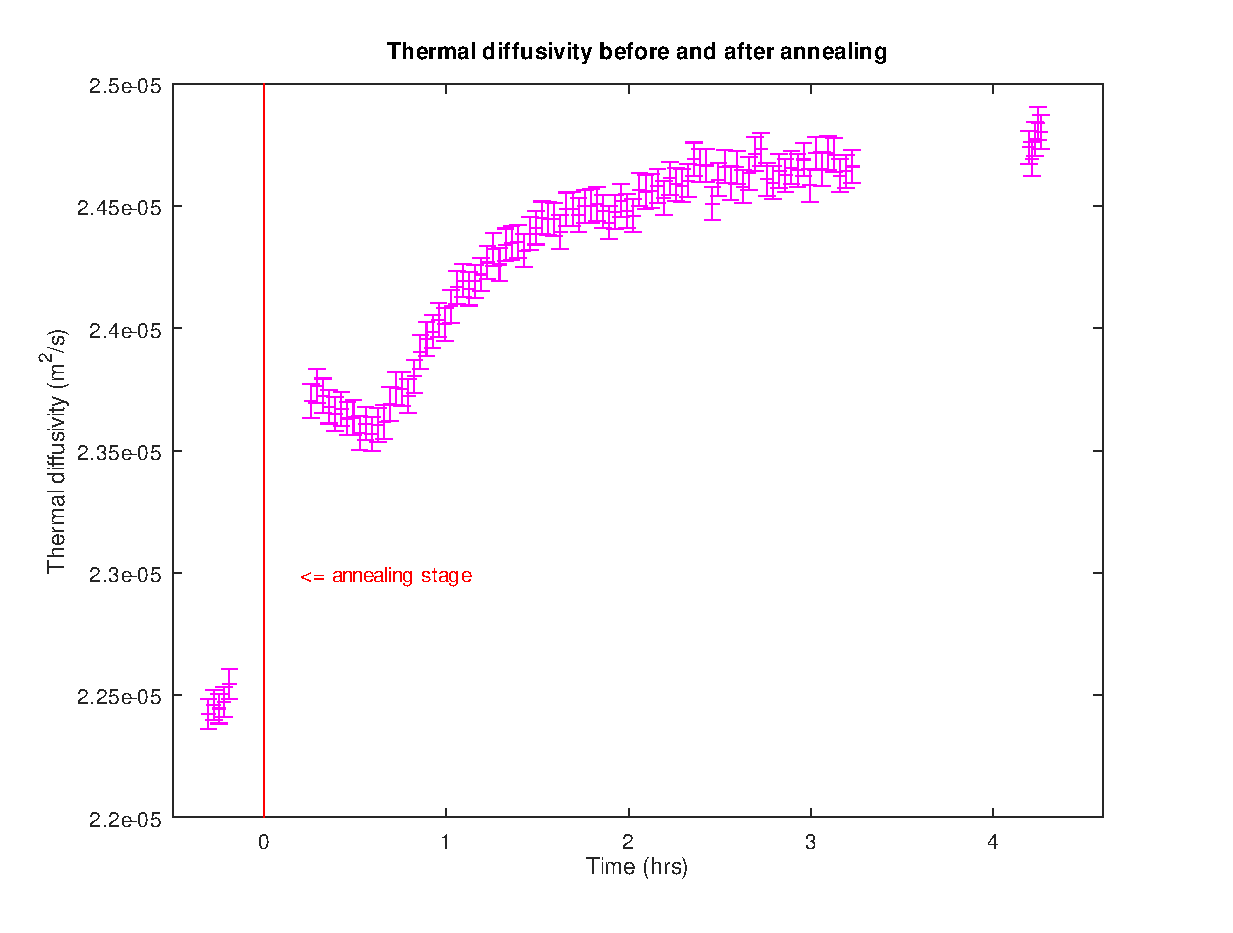
\includegraphics[width=\textwidth]{./images/thermal_diffusivity_pre_post.eps}
\caption{Thermal diffusivity results from TGS for entire experiment. Annealing stage is cut out for ease of comparing pre-annealing thermal diffusivity values (left of the red line) to post-annealing thermal diffusivity values (right of the red line). As radiation damage events per second are constant over the experiment, damage accumulates linearly with elapsed time since annealing.}
\label{thermal_diffusivity_pre_post}
\end{center}
\end{figure}

\begin{figure}[pt]
\begin{center}
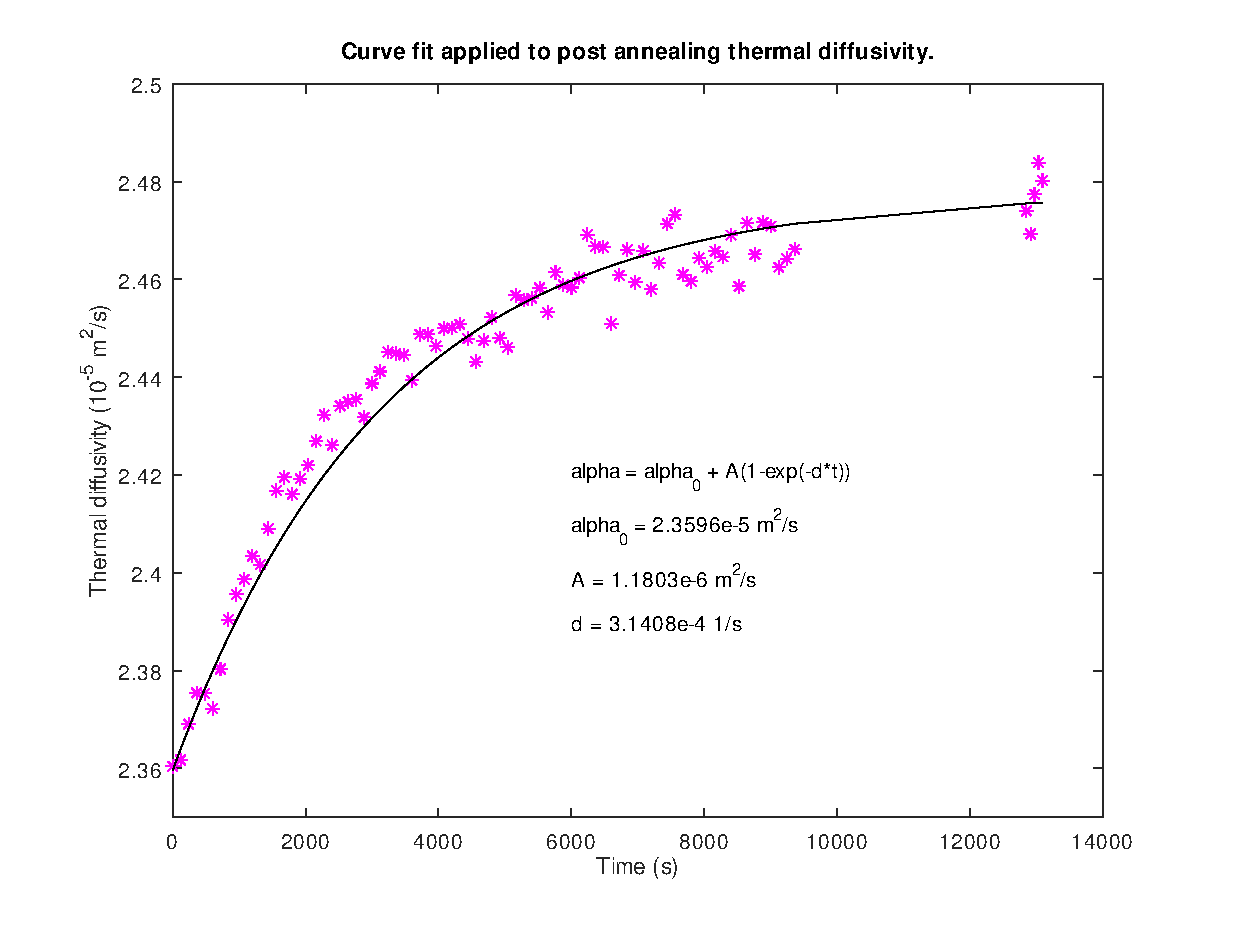
\includegraphics[width=\textwidth]{./images/curve_fit.eps} 
\caption{Generalized least squares fit to thermal diffusivity data after annealing and after ``hook''. Equation form chosen due to evidence that damage approaches a maximum.}
\label{curve_fit}
\end{center}
\end{figure}


\begin{figure}[pt]
\begin{center}
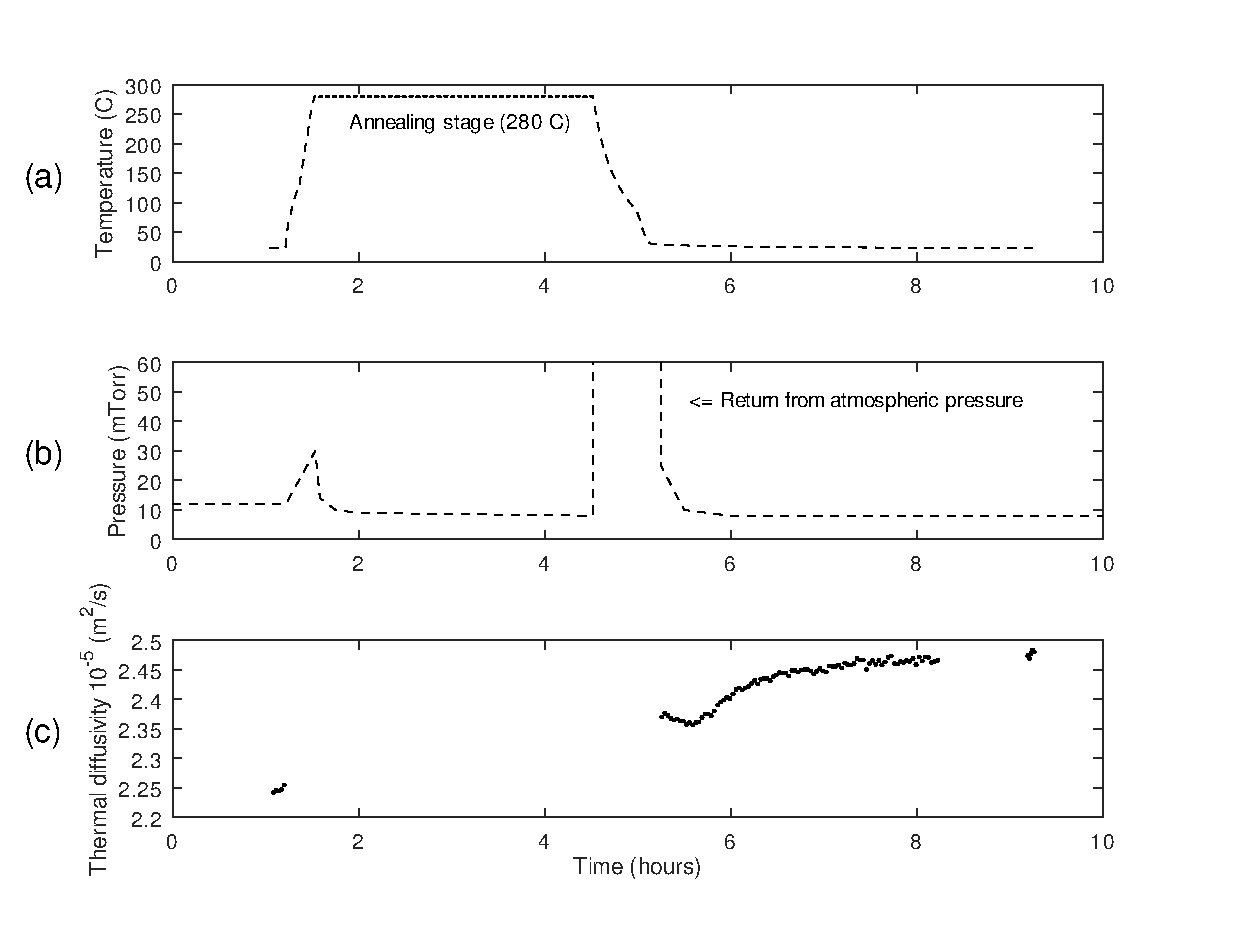
\includegraphics[width=\textwidth]{./images/T_P_alpha_subplots.eps}
\caption{Thermal diffusivity results from TGS are again plotted for the entire experiment in (c), but this time accompanied by the temperature record in (a) and the pressure record in (b) to clarify chronology of experiment. This also illustrates the coincidence between the pressure transient and the hook in the post-anneal thermal diffusivity data at $\sim$5.5 hours.}
\label{T_P_alpha_subplots}
\end{center}
\end{figure}


\begin{figure}[pt]
\begin{center}
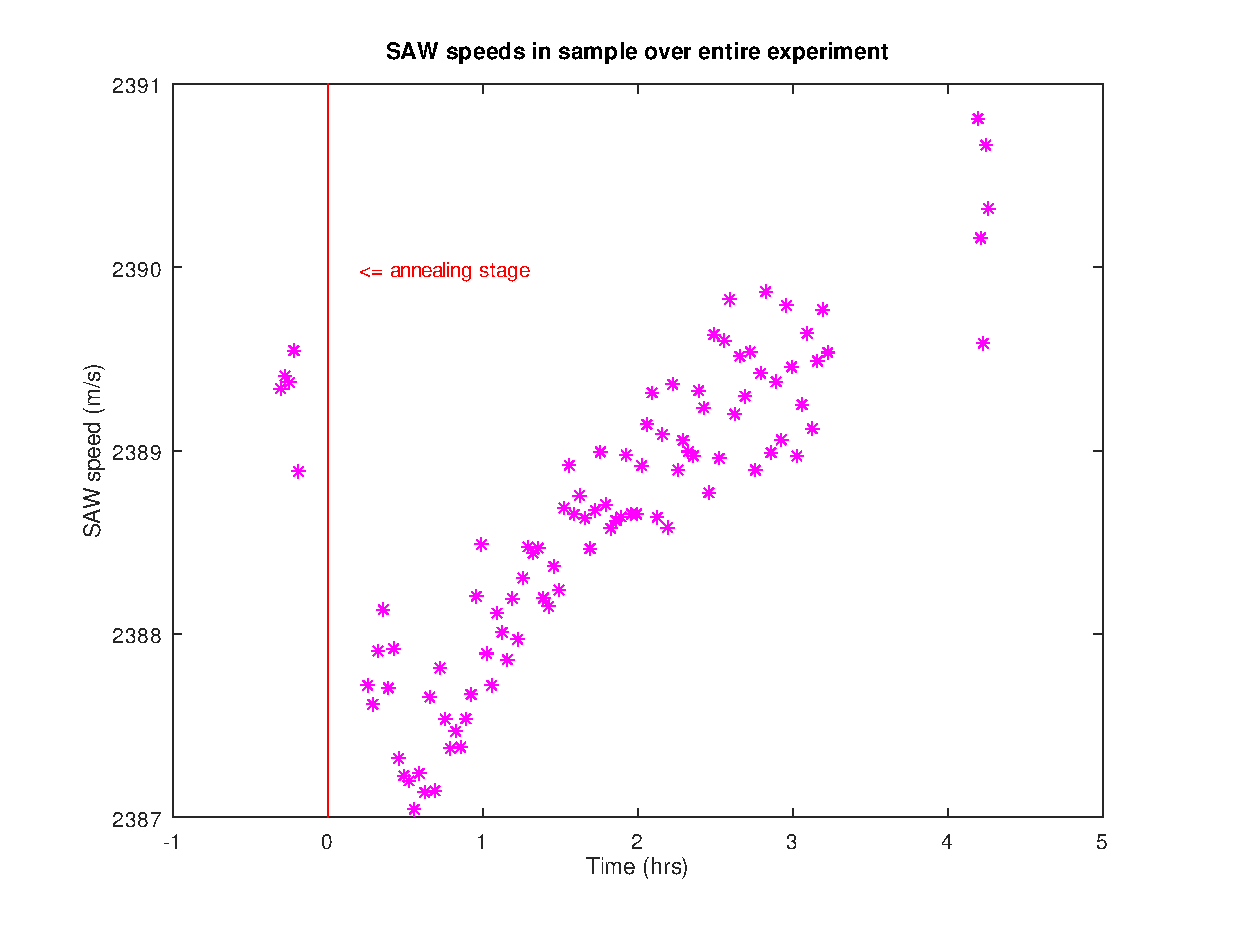
\includegraphics[width=\textwidth]{./images/SAW_speeds.eps}
\caption{SAW speed results from TGS are plotted for the entire experiment. The annealing stage is cut out so that pre and post annealing measurements can be compared more easily by eye. As SAW speed is proportional to elasticity, this plot indicates that annealing reduces stiffness caused by radiation damage, which immediately begins to accumulate again.}
\label{SAW_speeds}
\end{center}
\end{figure}




% \cite{patterson:risc,rad83}.  
% \cite{ellis:bulldog,pet87,coutant:precision-compilers}.  In these cases, the
% \cite{gib86}.
% These optimizations are described in detail in section~\ref{ch1:opts}.
% \section{Description of micro-optimization}\label{ch1:opts}
% \footnote{A description of the floating point format used is shown in figures~\ref{exponent-format}
% and~\ref{mantissa-format}.}.  
% A discussion of the mathematics behind unnormalized arithmetic is in appendix~\ref{unnorm-math}.

% \footnote{Using unnormalized numbers for math is not a new idea; a
% good example of it is the Control Data CDC 6600, designed by Seymour Cray.
% \cite{thornton:cdc6600} The CDC 6600 had all of its instructions performing
% unnormalized arithmetic, with a separate {\tt NORMALIZE} instruction.}.

% This is an example of how you would use tgrind to include an example
% of source code; it is commented out in this template since the code
% example file does not exist.  To use it, you need to remove the '%' on the
% beginning of the line, and insert your own information in the call.
%
%\tagrind[htbp]{code/pmn.s.tex}{Post Multiply Normalization}{opt:pmn}

% This is an example of how you would use tgrind to include an example
% of source code; it is commented out in this template since the code
% example file does not exist.  To use it, you need to remove the '%' on the
% beginning of the line, and insert your own information in the call.
%
%\tgrind[htbp]{code/be.s.tex}{Block Exponent}{opt:be}

%% This is an example first chapter.  You should put chapter/appendix that you
%% write into a separate file, and add a line \include{yourfilename} to
%% main.tex, where `yourfilename.tex' is the name of the chapter/appendix file.
%% You can process specific files by typing their names in at the 
%% \files=
%% prompt when you run the file main.tex through LaTeX.
\chapter{Conclusion}
The findings of this work, like so many, create more questions than they put to rest. 
SAW speed increases with radiation damage, and annealing can indeed heal this damage to restore SAW speed to that of the defect-free crystal. This makes for an unintentional confirmation of the findings of Dienes and Nabarro. It appears that thermal diffusivity, at least in lead sulfide thin films, also increases with radiation damage. This effect in particular warrants additional study, if only to determine the mechanism behind it.

Are new energy levels in the band gap liberating electrons in the short term, only to be swamped by the larger but latent effect of phonon scattering in the long term? Additional studies of radiation damage in PbS are necessary, wherein the sample is tested at logarithmically spaced time intervals. This could definitively rule out latent effects. A study of radiation damage's effect on band gap could also elucidate which new energy levels are available and how much they actually affect charge carrier mobility. An x-ray diffraction study could reveal the time evolution of the crystal lattice, which would measure more directly the amount of lattice amorphization that corresponds to the steady state damage condition this work was predicated on. 

Other potential follow up studies include both the simpler and the more complex. Affects of annealing and rapid pressure changes are unlikely but possible sources of effects on thermal diffusivity. It would be especially telling if a repetition of this experiment were carried out with several different annealing temperatures. One could rule out an affect of annealing temperature on elastic and thermal properties. An XRD study could potentially reveal if PbS, especially when doped with thorium, is cable of a previously unknown solid phase. Finally, a mathematically sophisticated but very necessary study must be carried out to deconvolve the respective contributions of the substrate and thin film to the signal captured by TGS when the grating spacing $\lambda$---and thus the interrogation depth---exceeds film thickness. Because quantum confinement is one most exciting features of thin films, future films to be studied with TGS will likely be thinner than 500 nm, not thicker.








%SAW speed increases with radiation damage
%Thermal diffusivity increases with radiation damage
%Does it come back down later?
%Did annealing cause a problem?
%Someone needs to follow up and do more TGS on aged sample
%Someone needs to do band gap measurements to realize true potential of self-irradiation
%Band gap changes might indicate any of these effects, especially the presence of additional energy levels in the gap.
%Someone needs to measure resistance



%Mike Short recommends these:
%G. J. Dienes, A theoretical estimate of the effect of radiation on the elastic constants of simple metals, Phys. Rev. 86, 228 (1952).
%F. R. N. Nabarro, Effect of radiation on elastic constants, Phys. Rev. 87, 665 (1952).
%G. J. Dienes, Effect of radiation on elastic constants, Phys. Rev. 87, 666 (1952).




%Although the findings laid out above are inconclusive in that (why are the inconclusive), they lay important groundwork for future iterations of these (describe tests). The results of my experiment indicate that (main finding), however in future experiments, researchers should be careful to (major thing that should be done differently next time). 
%(Thing I'm suggesting researches do differently next time) could lead to (suggest a finding if researchers follow your advice).
%(Another suggestion of what you think could be done differently next time) (A final suggestion of what you think could be done differently next time) 
%(A sentence stating your main finding and encouraging scientists to pick up where you left off.) (A sentence reiterating the limitations of your finding)


% \cite{patterson:risc,rad83}.  
% \cite{ellis:bulldog,pet87,coutant:precision-compilers}.  In these cases, the
% \cite{gib86}.
% These optimizations are described in detail in section~\ref{ch1:opts}.
% \section{Description of micro-optimization}\label{ch1:opts}
% \footnote{A description of the floating point format used is shown in figures~\ref{exponent-format}
% and~\ref{mantissa-format}.}.  
% A discussion of the mathematics behind unnormalized arithmetic is in appendix~\ref{unnorm-math}.

% \footnote{Using unnormalized numbers for math is not a new idea; a
% good example of it is the Control Data CDC 6600, designed by Seymour Cray.
% \cite{thornton:cdc6600} The CDC 6600 had all of its instructions performing
% unnormalized arithmetic, with a separate {\tt NORMALIZE} instruction.}.

% This is an example of how you would use tgrind to include an example
% of source code; it is commented out in this template since the code
% example file does not exist.  To use it, you need to remove the '%' on the
% beginning of the line, and insert your own information in the call.
%
%\tagrind[htbp]{code/pmn.s.tex}{Post Multiply Normalization}{opt:pmn}

% This is an example of how you would use tgrind to include an example
% of source code; it is commented out in this template since the code
% example file does not exist.  To use it, you need to remove the '%' on the
% beginning of the line, and insert your own information in the call.
%
%\tgrind[htbp]{code/be.s.tex}{Block Exponent}{opt:be}

\appendix
%\chapter{Tables}

\begin{table}
\caption{Armadillos}
\label{arm:table}
\begin{center}
\begin{tabular}{||l|l||}\hline
Armadillos & are \\\hline
our	   & friends \\\hline
\end{tabular}
\end{center}
\end{table}

\clearpage
\newpage

%\chapter{Figures}

\vspace*{-3in}

\begin{figure}
\vspace{2.4in}
\caption{Armadillo slaying lawyer.}
\label{arm:fig1}
\end{figure}
\clearpage
\newpage

\begin{figure}
\vspace{2.4in}
\caption{Armadillo eradicating national debt.}
\label{arm:fig2}
\end{figure}
\clearpage
\newpage

%% This defines the bibliography file (main.bib) and the bibliography style.
%% If you want to create a bibliography file by hand, change the contents of
%% this file to a `thebibliography' environment.  For more information 
%% see section 4.3 of the LaTeX manual.
\begin{singlespace}
\bibliography{main}
\bibliographystyle{unsrt}
\end{singlespace}

\end{document}

